
\documentclass[12pt]{report} 

\usepackage[croatian]{babel} 
\usepackage{amssymb}
\usepackage{amsmath}
\usepackage{txfonts}
\usepackage{mathdots}
\usepackage{titlesec}
\usepackage{array}
\usepackage{lastpage}
\usepackage{etoolbox}
\usepackage{longtable, tabu}
\usepackage{color, colortbl}
\usepackage{adjustbox}
\usepackage{geometry}
\usepackage[classicReIm]{kpfonts}
\usepackage{hyperref}
\usepackage{fancyhdr}

\usepackage{float}
\usepackage{setspace}
\restylefloat{table}


\patchcmd{\chapter}{\thispagestyle{plain}}{\thispagestyle{fancy}}{}{}


\titleformat{\chapter}{\normalfont\huge\bfseries}{\thechapter.}{20pt}{\Huge}
\titlespacing{\chapter}{0pt}{0pt}{40pt}
\linespread{1.3}

\geometry{
	a4paper,
	left=1in,
	top=1in,
}

\hypersetup{ colorlinks, citecolor=black, filecolor=black, linkcolor=black,	urlcolor=black }


\newenvironment{packed_enum}{
	\begin{enumerate}
		\setlength{\itemsep}{0pt}
		\setlength{\parskip}{0pt}
		\setlength{\parsep}{0pt}
	}{\end{enumerate}}

\newenvironment{packed_item}{
	\begin{itemize}
		\setlength{\itemsep}{0pt}
		\setlength{\parskip}{0pt}
		\setlength{\parsep}{0pt}
	}{\end{itemize}}


\definecolor{LightBlue}{rgb}{0.9,0.9,1}
\definecolor{LightGreen}{rgb}{0.9,1,0.9}


%podesavanje headera i footera


\pagestyle{fancy}
\lhead{Oblikovanje programske potpore}
\rhead{Internet bankarstvo}
\lfoot{BugBusters}
\cfoot{stranica \thepage/\pageref{LastPage}}
\rfoot{\today}
\renewcommand{\headrulewidth}{0.2pt}
\renewcommand{\footrulewidth}{0.2pt}


\begin{document}
	

	\begin{titlepage}
		\begin{center}
			\vspace*{\stretch{1.0}}
			\LARGE Oblikovanje programske potpore\\
			\large Ak. god. 2019./2020.\\
			
			\vspace*{\stretch{3.0}}
			
			\huge Internet bankarstvo\\
			\Large Dokumentacija, Rev. \textit{$<$1 ili 2$>$}\\
			
			\vspace*{\stretch{12.0}}
			\normalsize
			Grupa: \textit{BugBusters}\\
			Voditelj: \textit{Matija Bačić}\\
			
			
			\vspace*{\stretch{1.0}}
			Datum predaje: \textit{$<$dan$>$. $<$mjesec$>$. $<$godina$>$.}\\
	
			\vspace*{\stretch{4.0}}
			
			Nastavnik: \textit{Hrvoje Nuić}\\
		
		\end{center}

	
	\end{titlepage}

	
	\tableofcontents

	\chapter{Dnevnik promjena dokumentacije}
				
		
		\begin{longtabu} to \textwidth {|X[2, l]|X[13, l]|X[3, l]|X[3, l]|}
			\hline \multicolumn{1}{|l|}{\textbf{Rev.}}	& \multicolumn{1}{l|}{\textbf{Opis promjene/dodatka}} & \multicolumn{1}{|l|}{\textbf{Autori}} & \multicolumn{1}{l|}{\textbf{Datum}} \\[3pt] \hline
			\endfirsthead
			
			\hline \multicolumn{1}{|l|}{\textbf{Rev.}}	& \multicolumn{1}{l|}{\textbf{Opis promjene/dodatka}} & \multicolumn{1}{|l|}{\textbf{Autori}} & \multicolumn{1}{l|}{\textbf{Datum}} \\[3pt] \hline
			\endhead
			
			\hline 
			\endlastfoot
			
			0.1 & Napravljen predložak.	& Bačić & 15.10.2019. 		\\[3pt] \hline 
			0.2	& Dodani funkcionalni zahtjevi. & Milošević & 17.10.2019. 	\\[3pt] \hline 
			0.3	& Dodani obrasci uporabe. & Bastalić \newline Gudelj & 20.10.2019. 	\\[3pt] \hline 
			0.4	& Dodani ostali zahtjevi. & Vučemilo & 21.10.2019. 	\\[3pt] \hline 
			0.5	& Dodan opis projektnog zadatka. & Bačić & 22.10.2019. 	\\[3pt] \hline 
			0.6	& Nadopuna i ispravak funkcionalnih zahtjeva. & Milošević & 22.10.2019. 	\\[3pt] \hline 
			0.7	& Dopuna i ispravak obrazaca uporabe. & Bastalić \newline Gudelj & 24.10.2019. 	\\[3pt] \hline 
			\textbf{1.0} & Verzija samo s bitnim dijelovima za 1. ciklus & Bačić & 01.01.1970. \\[3pt] \hline
			\textbf{2.0} & Konačni tekst predloška dokumentacije  & Bačić & 01.01.1970. \\[3pt] \hline 
			&  &  & \\[3pt] \hline
			
			
		\end{longtabu}
	\chapter{Opis projektnog zadatka}
		
		Potreba za kvalitetnom digitalizacijom bankarskih procesa i uvid u stanje pojedinih računa iz udobnosti doma od velikog su značaja kako za klijente, tako i za djelatnike banke. Cilj je ovog projekta razviti bankarski sustav: bazu podataka i sučelja prema bankarima, administratorima te krajnjim korisnicima banke, odnosno građanima.
		Korisnike dijelimo u nekoliko skupina : 
		\begin{packed_item}
			\item \textbf{administratori}, 
			\item \textbf{bankari},
			\item \textbf{službenici za odobravanje kreditnih zahtjeva građana} i 
			\item \textbf{korisnici u užem smislu} (građani).
		\end{packed_item}
		
		Svaka vrsta korisnika sustava ima svoj jedinstveni pogled u sustav putem web sučelja i Android aplikacije.
		
		\textit{\textbf{Neregistrirani korisnik}}, za registraciju u sustav upisuje svoj OIB i jedinstveni ključ koji je dobio od bankara. Nakon uspješnog unosa tih podataka, odabire korisničko ime i lozinku koji će mu u buduće služiti za prijavu u sustav. Ostale podatke o pojedinom korisniku kao što su: ime, prezime, adresa prebivališta, datum rođenja, e-mail adresa, sliku korisnika i dr., u sustav unosi bankarski službenik prilikom ugovaranja bilo kakve usluge banke.
		
		\textit{\textbf{Administrator}} u sustav ulazi putem unaprijed definirane web adrese gdje unosi svoje korisničko ime i lozinku koji mu daju pristup sustavu. On vidi popis svih korisnika sustava te može uređivati podatke za bilo koju vrstu korisnika, kao i dodavati te brisati same korisnike sustava. Jedina je osoba koja može kreirati račune ostalim djelatnicima banke.
		
		\textit{\textbf{Bankar}} svoj korisnički račun dobivaju od administratora. Ime, prezime, adresa prebivališta, OIB, datum rođenja, e-mail adresa i slika profila unaprijed su poznati podaci koje u sustav unosi administrator za svakog novog djelatnika. Pošto postanu dio kolektiva banke te nakon što administrator unese njihove podatke u sustav, u web aplikaciju unose korisničko ime i privremenu lozinku dobivenu od administratora sustava. Nakon prijave privremenom lozinkom, obavezni su odmah stvoriti novu lozinku. U sustavu imaju uvid u sve svoje osobne podatke, ali nemaju mogućnost izmjene tih podataka.
		Bankar nema uvid u popis korisnika sustava, niti u popis klijenata banke (građana). On može otvoriti, obrisati ili mijenjati profile klijenata. Kako bi pronašao profil nekog građana i uređivao ga ili brisao, dužan je unijeti OIB osobe za koju radi izmjenu u sustavu nakon čega mu se otvara profil te osobe (pretraga profila radi se po OIB-u građana). Također mu je dozvoljeno otvarati i zatvarati tekuće, žiro, štedne račune, ugovarati kredite, kreditne i debitne kartice za korisnike banke, aktivacija i deaktivacija kartica te obavljanje transakcija po računima klijenata.
		
		Svaki tekući račun ima dozvoljeno prekoračenje, a svaka kreditna kartica ima ugovoren limit.
		
		\textit{\textbf{Klijent}} dobiva dozvolu pristupa sustavu od bankara. Klijent banke ima uvid u sve podatke o svom profilu (ime, prezime, OIB, prebivalište, datum rođenja, slika profila i drugo), ali ih ne može mijenjati. Također, klijent može vidjeti sve svoje transakcijske račune, štedne račune, ugovorene kredite i kartice (debitne i kreditne). Klijent ne može mijenjati osobne podatke, podatke o računima, kreditima ili karticama. Klijent može vršiti prijenos sredstava između svojih računa transakcijskih računa (tekućeg, žiro ili štednog) ili na račune drugih klijenata banke. Također, klijent može ručno izvršiti uplatu kredit ili na kreditnu karticu kako bi umanjio iznos dugovanja ili otplatiti dugovanje ukupno.
		Klijent podnosi zahtjev za kreditom ili kreditnom karticom putem aplikacije ili u poslovnici banke gdje taj zahtjev unosi bankarski službenik. Za izradu kreditnog zahtjeva, u sustav se unosi iznos kredita, namjena kredita i rok otplate, dok kamatna stopa ovisi isključivo o namjeni kredita. Za izradu zahtjeva za kreditnom karticom, u sustav je potrebno unijeti samo vrstu kartice koja se traži (Mastercard, Visa, American Express, Diners, Discover i dr.).
		
		Svi korisnici moraju imati sliku profila (standardna slika za osobnu iskaznicu).
		
		Jednom mjesečno, u web aplikaciji, korisniku dolazi izvod po svim transakcijskim računima i kreditnim karticama u PDF i XLS obliku.
		
		Također, potrebno je da banka ima definirane poslovnice. Svaka poslovnica u sustavu ima ime poslovnice, adresu poslovnice i jedinstveni identifikator. Svaki djelatnik banke vezan je za jednu od poslovnica. Dodatno, svaki klijent može zatražiti sastanak u određenoj poslovnici u određeno vrijeme u budućnosti kojeg preuzima neki od slobodnih bankara te poslovnice. Nakon što bankar odobri sastanak, klijentu u web sučelje dolazi obavijest u kojoj je navedeno ime poslovnice, adresa poslovnice, ime bankara te datum i vrijeme zakazanog sastanka.
		
		\textit{\textbf{Službenici za odobravanje kreditnih zahtjeva građana}} imaju uvid u svoje osobne podatke koje ne mogu mijenjati. Također, vidljivi su im svi neobrađeni kreditni zahtjevi svih klijenata banke. Službenik može preuzeti bilo koji zahtjev na obradu te tada ima uvid u podatke o zahtjevu i sve podatke o klijentu koje banka posjeduje. Podaci o zahtjevu sadrže iznos zatraženog kredita, namjena kredita, kamatna stopa i vrijeme otplate ako se radi o zahtjevu za kredit, odnosno vrsta zatražene kreditne kartice ako se radi o zahtjevu za kreditnom karticom. Jedini podatak od navedenih koji se ne može mijenjati jest kamatna stopa jer ona ovisi o namjeni kredita. Službenik tada odobrava ili odbija zahtjev za kreditom, odnosno odobrava ili odbija kreditnu karticu kojoj ručno stvara određeni limit i kamatnu stopu.
		Nakon donesene odluke, korisnik tu odluku vidi u aplikaciji.
		
		Rate za kredite i kreditne kartice klijenata skidaju se automatski svaki mjesec na datum kojeg odredi administrator sustava i on je jedinstven za sve. U slučaju da na tekućem računu korisnika ne postoji dovoljno sredstava, ta se rata odgađa za jedan mjesec i bit će naplaćena zajedno s novom ratom idući mjesec.
		
		Debitne kartice u sustavu prikazuju se odvojeno od tekućeg ili žiro računa kojem pripadaju. Može postojati račun bez debitne kartice, ali ne i debitna kartica bez računa. Odnosno, svaka debitna kartica mora biti vezana uz jedan račun.
		
		Primjeri ovakvog sustava mogu se pronaći u svim modernim, vodećim bankama u svijetu i u Hrvatskoj. Neki od njih prikazani su u nastavku.
		
		\begin{figure}[H]
			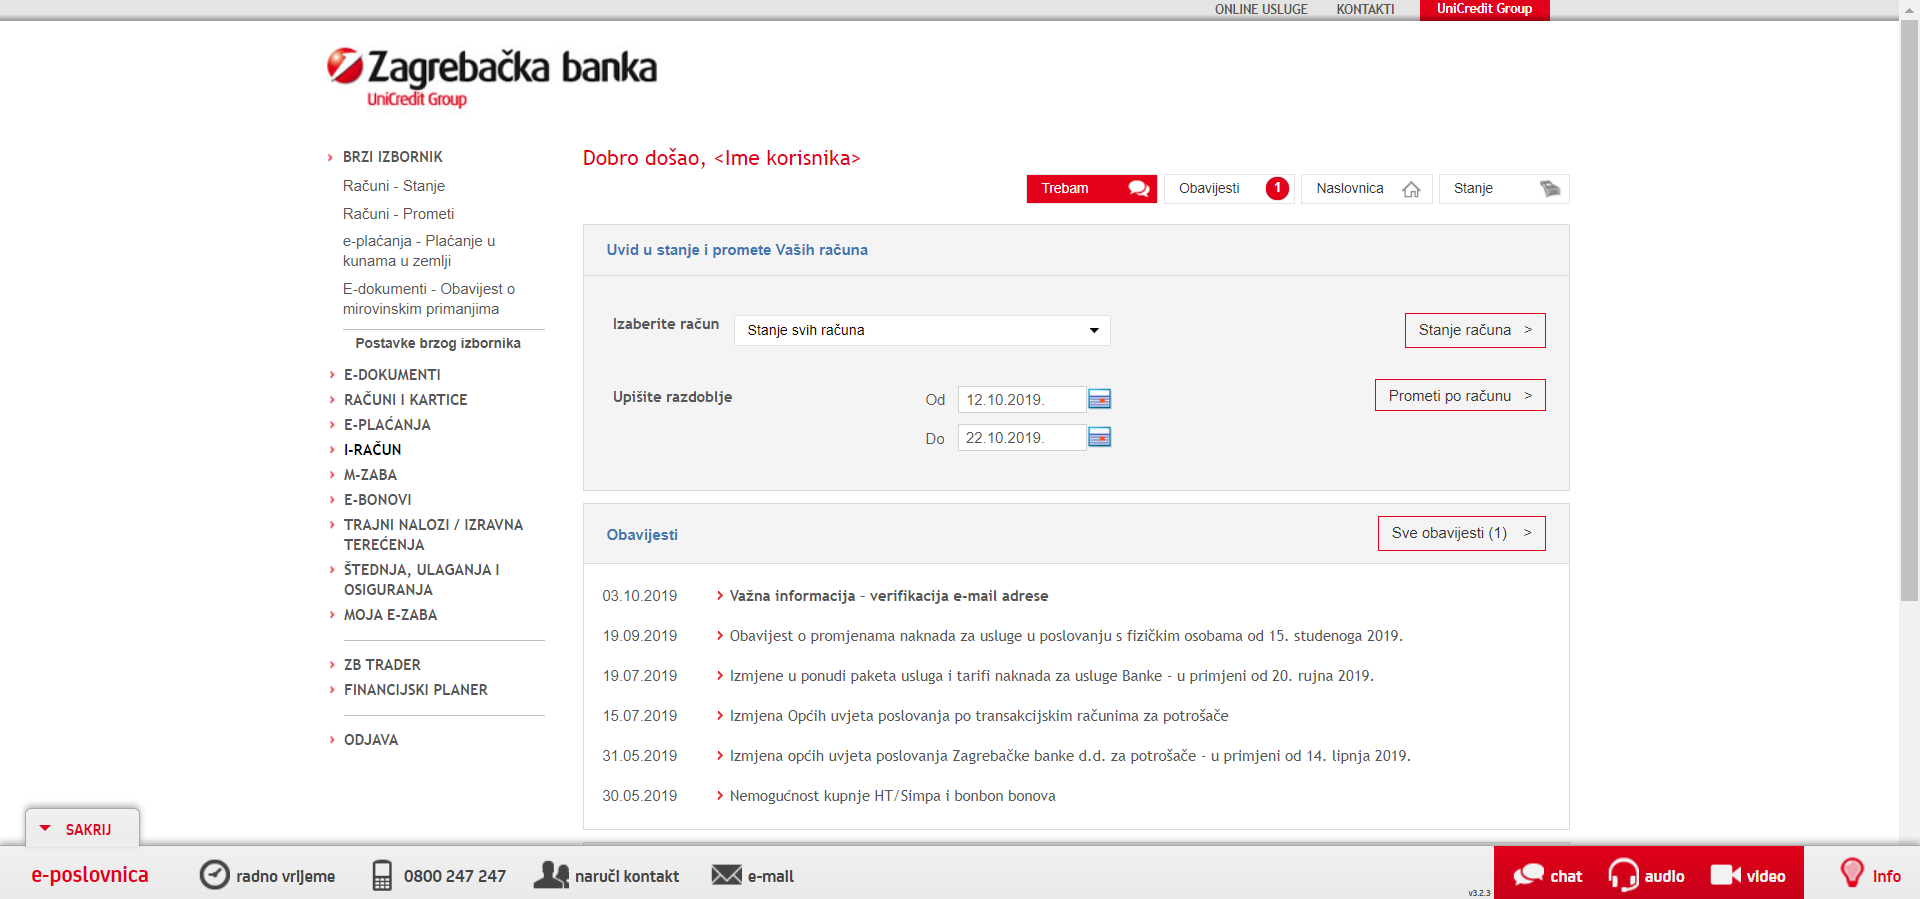
\includegraphics[scale=0.4]{slike/ezaba.PNG}
			\centering
			\caption{Usluga internet bankarstva Zagrebačke banke}
			\label{fig:ezaba}
		\end{figure}
	
		\begin{figure}[H]
			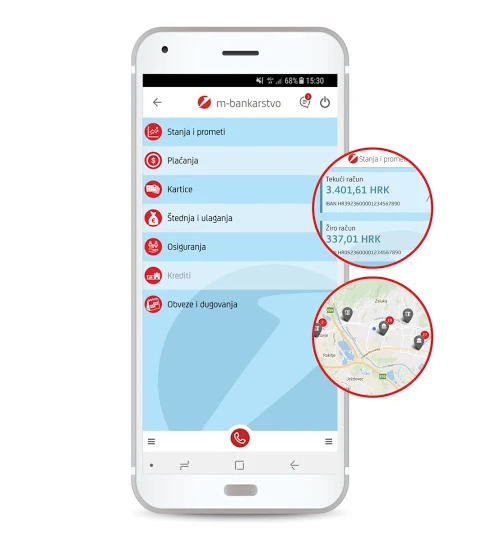
\includegraphics[scale=1]{slike/mzaba.PNG}
			\centering
			\caption{Usluga mobilnog bankarstva Zagrebačke banke}
			\label{fig:mzaba}
		\end{figure}
	
		\begin{figure}[H]
			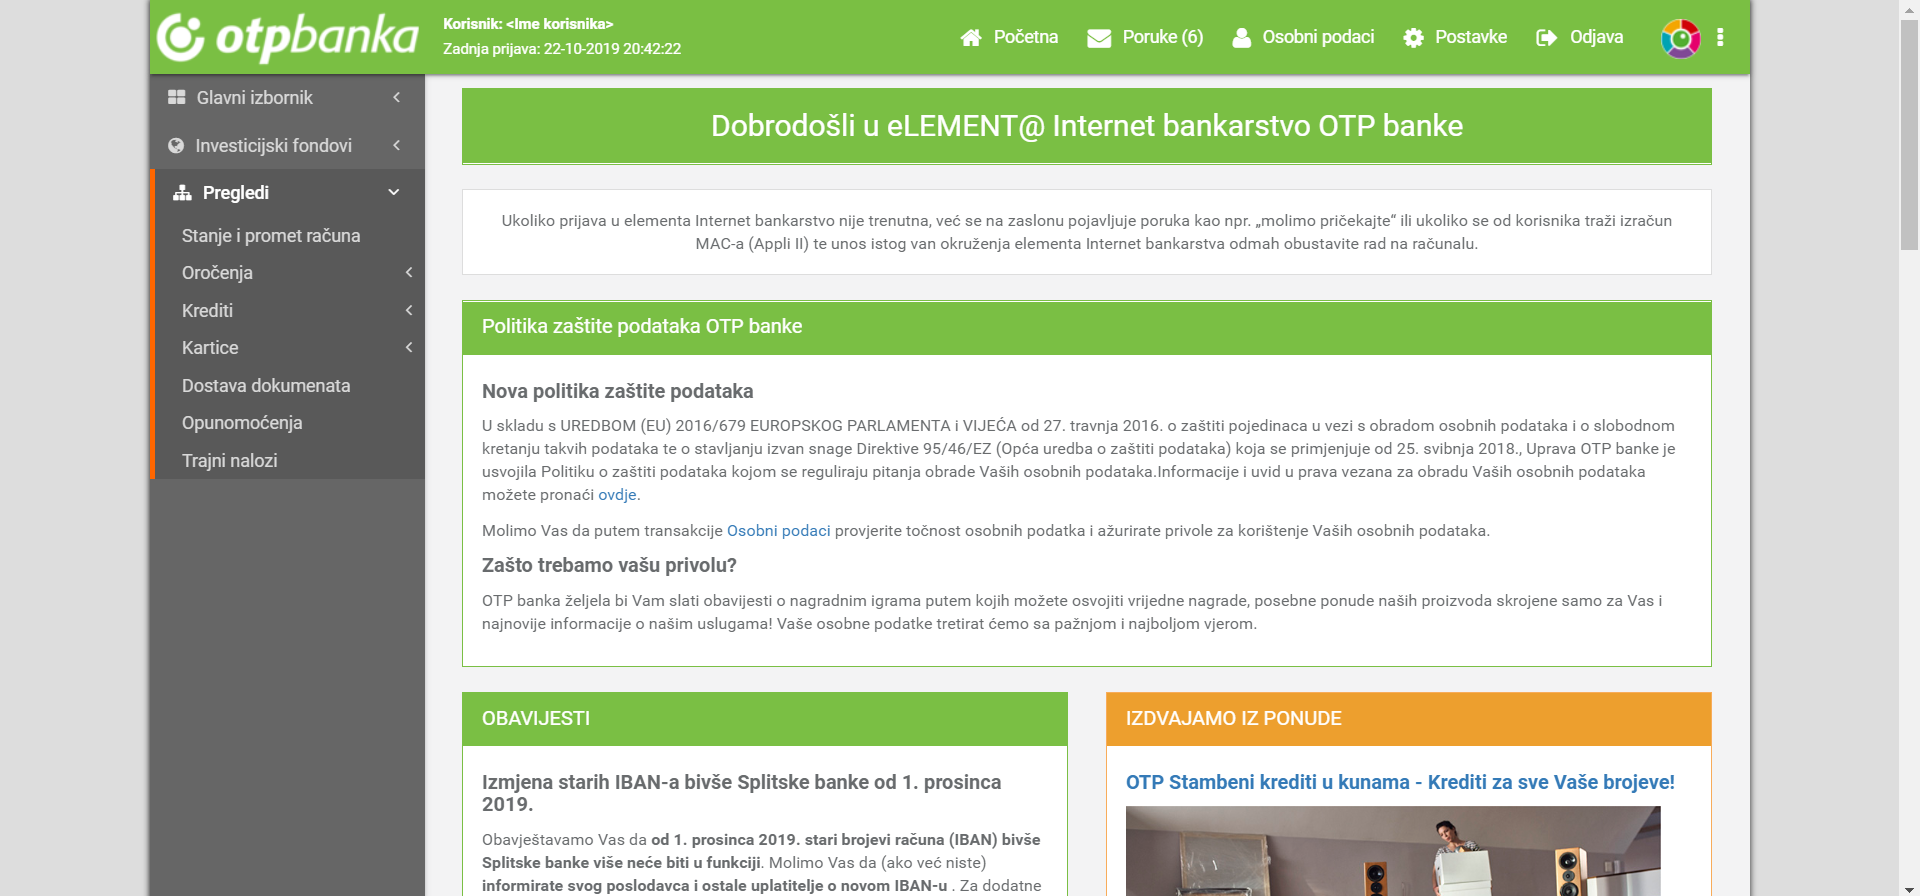
\includegraphics[scale=0.4]{slike/otp.PNG}
			\centering
			\caption{Usluga internet bankarstva OTP banke}
			\label{fig:otp}
		\end{figure}
		
		\eject
	\chapter{Specifikacija programske potpore}
		
	\section{Funkcionalni zahtjevi}
			
			
			\noindent \textbf{Dionici:}
			
			\begin{packed_enum}
				
				\item Banka
				\item Administrator sustava
				\item Službenici banke
				\begin{packed_enum}
					\item Bankari
					\item Službenici za odobravanje kredita građana
				\end{packed_enum}
				\item Klijenti banke
				
			\end{packed_enum}
			
			\noindent \textbf{Aktori i njihovi funkcionalni zahtjevi:}
			
			
			\begin{packed_enum}
				\item  \underbar{Administrator - inicijator}
				
				\begin{packed_enum}
					
					\item Pristup sustavu pomoću korisničkog imena i lozinke
					\item Pregled popisa svih profila i uz njih vezanih korisničkih računa
					\item Dodavanje novih profila u sustav
					\begin{packed_enum}
						\item Unosi ime, prezime, adresu prebivališta, OIB, datum rođenja, e-mail adresu, sliku profila, vrsta korisnika
					\end{packed_enum}
					\item Izmjena podataka profila i mijenjanje razine pristupa korisnicima aplikacije
					\item Brisanje profila korisnika
					\item Dodavanje novog korisničkog računa
					\begin{packed_enum}
						\item Odabir korisničkog imena, sustav generira privremenu lozinku koju je potrebno promijeniti prilikom prve prijave
					\end{packed_enum}
					\item Brisanje korisničkog računa pojedinih profila
					
				\end{packed_enum}
			\eject
				\item  \underbar{Baza podataka - sudionik}
				
				\begin{packed_enum}
					
					\item Sadrži podatke o profilima korisnika sustava
					\begin{packed_enum}
						\item Ime, prezime, adresa, OIB, datum rođenja, e-mail adresa, slika profila, vrsta korisnika
						\item Sve korisničke račune vezane za jedan profil
					\end{packed_enum}
					\item Sadrži podatke o računima klijenata
					\begin{packed_enum}
						\item Broj i stanje tekućeg računa
						\item Broj i stanje žiro računa
						\item Broj i stanje štednog računa
					\end{packed_enum}
					\item Sadrži podatke o karticama klijenata
					\begin{packed_enum}
						\item Broj i vrsta kartice
						\begin{packed_enum}
							\item Debitna kartica - vezana uz račun
							\item Kreditna kartica - nije vezana uz račun
						\end{packed_enum}
						\item Ukoliko je kartica kreditna, sadrži ukupno dugovanje i ukupni odobreni limit po kartici
					\end{packed_enum}
					\item Sadrži podatke o transakcijama među računima klijenata banke
					\item Sadrži podatke o transakcijama po debitnim i kreditnim karticama
					\item Sadrži podatke o kreditima
					\begin{packed_enum}
						\item Iznos, namjena, rok otplate kredita u mjesecima i kamatna stopa
						\item Ukupno preostalo dugovanje (u početku jest iznos uvećan za kamatnu stopu, smanjuje se s otplatom)
					\end{packed_enum}
					
				\end{packed_enum}
				
				\item	\underbar{Bankar - inicijator}
				
				\begin{packed_enum}
					
					\item Inicijalnu prijavu u sustav vrši pomoću korisničkog imena i privremene lozinke dobivene od administratora
					\begin{packed_enum}
						\item Nakon inicijalne prijave obvezan je odmah stvoriti novu lozinku
					\end{packed_enum}
					\item Mogućnost uvida u vlastiti profil
					\begin{packed_enum}
						\item Ime, prezime, adresa, OIB, datum rođenja, e-mail adresa, slika profila
					\end{packed_enum}
					\item Izrada korisničkih profila klijenata banke
					\begin{packed_enum}
						\item Unosi ime, prezime, adresu, OIB, datum rođenja, e-mail adresu, sliku profila klijenta
					\end{packed_enum}
					\item Brisanje korisničkih profila klijenata
					\item Izmjena podataka u korisničkim profilima klijenata
					\item Pretraga profila klijenata pomoću OIB-a klijenta
					\item Otvaranje i zatvaranje tekućih, žiro i štednih računa
					\item Obavljanje transakcija po računima klijenata
					\item Ugovaranje, aktivacija i deaktivacija debitnih i kreditnih kartica
					\item Ugovaranje kredita
					\item Otvaranje korisničkih računa za profile klijenata
					\begin{packed_enum}
						\item Otvaranjem korisničkih računa dobiva prikaz privremenog ključa kojeg korisnik unosi uz svoj OIB kako bi odabrao korisničko ime i lozinku
					\end{packed_enum}
					\item Brisanje korisničkih računa za profile klijenata
					
				\end{packed_enum}
			
				\item	\underbar{Službenik za odobravanje kreditnih zahtjeva - sudionik}
				
				\begin{packed_enum}
					
					\item Inicijalnu prijavu u sustav vrši pomoću korisničkog imena i privremene lozinke dobivene od administratora
					\begin{packed_enum}
						\item Nakon inicijalne prijave obvezan je odmah stvoriti novu lozinku
					\end{packed_enum}
					\item Mogućnost uvida u vlastiti profil
					\begin{packed_enum}
						\item Ime, prezime, adresa, OIB, datum rođenja, e-mail adresa, slika profila
					\end{packed_enum}
					\item Odobrenje i blokiranje kreditnih zahtjeva
					\item Uvid u sve podatke o profilima klijentima čiji zahtjevi za kreditom nisu riješeni
					
				\end{packed_enum}
				
				\item	\underbar{Klijent banke - inicijator}
				
				\begin{packed_enum}
					
					\item Pregledavanje podataka isključivo o vlastitom profilu
					\begin{packed_enum}
						\item Ime, prezime, OIB, adresa, datum rođenja, e-mail adresa, slika profila
						\item Sve ugovorene usluge banke (transakcijski računi, krediti, debitne i kreditne kartice, štedni računi i dr.)
					\end{packed_enum}
					\item Pregledavanje podataka o transakcijama
					\item Prijenos sredstava između vlastitih računa
					\item Prijenos sredstava na račun drugih klijenata
					\item Može ručno izvršiti uplatu kredita ili uplatu na kreditnu karticu kako bi umanjio iznos duga ili kako bi otplatio sveukupno dugovanje
					\item Podnošenje zahtjeva za kreditom
					\begin{packed_enum}
						\item Unosi iznos i namjenu kredita, te rok otplate
					\end{packed_enum}
					\item Podnošenje zahtjeva za kreditnom karticom
					\begin{packed_enum}
						\item Unos vrste kartice (Mastercard, Visa, American Express, Diners, Discover)
					\end{packed_enum}
					
				\end{packed_enum}
				
				\item	\underbar{Neregistrirani korisnik - inicijator}
				
				\begin{packed_enum}
					
					\item Upisuje OIB i jedinstveni ključ dobiven od bankara kako bi se registrirao u sustav
					\item Nakon registracije odabire korisničko ime i lozinku koji će mu služiti za buduće prijave u sustav
					
				\end{packed_enum}
			
			\end{packed_enum}
			
			\eject 
			
			
				
			\subsection{Obrasci uporabe}
				
				\subsubsection{Opis obrazaca uporabe}
				
					\noindent \underbar{\textbf{UC1-Prijava u sustav }}
				\begin{packed_item}
					
					\item \textbf{Glavni sudionik: } Svi korisnici sustava
					\item  \textbf{Cilj:} Dobiti pristup sustavu
					\item  \textbf{Sudionici:} Baza podataka
					\item  \textbf{Preduvjet:} Korisnik ima korisnički račun
					\item  \textbf{Opis osnovnog tijeka:}
					
					\item[] \begin{packed_enum}
						
						\item Korisnik sustava unosi korisničko ime i lozinku
						\item Potvrda o ispravnosti korisničkih podataka
						\item Korisnik sustava dobiva pristup sustavu
						
					\end{packed_enum}
					
					\item  \textbf{Opis mogućih odstupanja:}
					
					\item[] \begin{packed_item}
						
						\item[2.a] Unos neispravnih podataka
						\item[] \begin{packed_enum}
							
							\item Ispis odgovarajuće poruke upozorenja 
							
							
						\end{packed_enum}
						
						
					\end{packed_item}
				\end{packed_item}
			
			
				\noindent \underbar{\textbf{UC2-Pregled profila svih korisnika sustava }}
				\begin{packed_item}
					
					\item \textbf{Glavni sudionik:} Administrator
					\item  \textbf{Cilj:} Pregledati registrirane korisnike i njihove osobne podatke
					\item  \textbf{Sudionici:} Baza podataka
					\item  \textbf{Preduvjet:} : Korisnik je registriran i dodijeljena su mu prava administratora
					\item  \textbf{Opis osnovnog tijeka:}
					
					\item[] \begin{packed_enum}
						
						\item Administrator odabire opciju pregledavanja korisnika
						\item Prikazuje se lista svih profila korisnika
						
					\end{packed_enum}
					
				\end{packed_item}
				
				
				
				
				
		   	\noindent \underbar{\textbf{UC3-Dodavanje novih profila u sustav }}
				\begin{packed_item}
						
						\item \textbf{Glavni sudionik: }Administrator
						\item  \textbf{Cilj:} Dodati profil u sustav
						\item  \textbf{Sudionici:} Baza podataka
						\item  \textbf{Preduvjet:} Profil se ne nalazi u bazi podataka
						\item  \textbf{Opis osnovnog tijeka:}
						
						\item[] \begin{packed_enum}
							
							\item Administrator unosi potrebne osobne podatke
							\begin{packed_enum}
								\item Ime, prezime, adresa, OIB, datum rodenja, e-mail adresa, slika profila, vrsta korisnika (razina pristupa sustavu)
							\end{packed_enum}
							\item Podaci se unose u bazu podataka
							\item Stvoren je novi profil
							
						\end{packed_enum}
						
						\item  \textbf{Opis mogućih odstupanja:}
						
						\item[] \begin{packed_item}
							
							\item[1.a] Unos neispravnih podataka (krivi OIB, profil s tim OIB-om ime već postoji i dr.)
							\item[] \begin{packed_enum}
								
								\item Ispis odgovarajuće poruke upozorenja
								
							\end{packed_enum}
							
						\end{packed_item}
					\end{packed_item}
				
				
				\noindent \underbar{\textbf{UC4-Izmjena podataka profila korisnika  }}
				\begin{packed_item}
					
					\item \textbf{Glavni sudionik: }Administrator
					\item  \textbf{Cilj:} Urediti i izmijeniti podatke profila
					\item  \textbf{Sudionici:} Baza podataka
					\item  \textbf{Preduvjet:} Korisnik je prijavljen u sustav kao administrator
					\item  \textbf{Opis osnovnog tijeka:}
					
					\item[] \begin{packed_enum}
						
						\item Administrator otvara željeni profil iz popisa svih korisnika
						\item Administrator odabire opciju uređivanja profila
						\item Administrator izmjenjuje podatke korisnika i sprema ih u bazu podataka 
						
					\end{packed_enum}
					
					
				\end{packed_item}
			
			
			\noindent \underbar{\textbf{UC5-Brisanje profila korisnika }}
			\begin{packed_item}
				
				\item \textbf{Glavni sudionik: }Administrator
				\item  \textbf{Cilj:} Obrisati korisnika
				\item  \textbf{Sudionici:} Baza podataka
				\item  \textbf{Preduvjet:} Korisnik je prijavljen u sustav kao administrator
				\item  \textbf{Opis osnovnog tijeka:}
				
				\item[] \begin{packed_enum}
					
					\item Administrator otvara željeni profil iz popisa svih korisnika
					\item Administrator odabire opciju brisanja profila
					\item Uklanja se korisnik i njegovi podaci iz baze podataka
					
				\end{packed_enum}
				
				
			\end{packed_item}
				
							
			
			\noindent \underbar{\textbf{UC6 - Promjena razine pristupa profila }}
			\begin{packed_item}
				
				\item \textbf{Glavni sudionik: }Administrator
				\item  \textbf{Cilj:} Promijeniti razinu pristupa korisnika sustavu (administrator, bankar, službenik za odobravanje kreditnih zahtjeva klijenata, klijent banke)
				\item  \textbf{Sudionici:} Baza podataka
				\item  \textbf{Preduvjet:} Korisnik je prijavljen u sustav kao administrator
				\item  \textbf{Opis osnovnog tijeka:}
				
				\item[] \begin{packed_enum}
					
					\item Administrator odabire željenog korisnika s popisa profila
					\item Izmijeni razinu pristupa korisnika
					
					
				\end{packed_enum}
				
			\end{packed_item}
			
			\noindent \underbar{\textbf{UC7 - Dodavanje novog korisničkog računa }}
			\begin{packed_item}
				
				\item \textbf{Glavni sudionik: }Administrator
				\item  \textbf{Cilj:} Dozvoliti pristup sustavu nekom korisniku
				\item  \textbf{Sudionici:} Baza podataka
				\item  \textbf{Preduvjet:} Korisnik je prijavljen u sustav kao administrator, postoji profil korisnika kome želimo dodati korisnički račun
				\item  \textbf{Opis osnovnog tijeka:}
				
				\item[] \begin{packed_enum}
					
					\item Administrator otvara željeni profil iz popisa svih korisnika
					\item Administrator odabire opciju dodavanja korisničkog računa
					\item Administrator odabire korisničko ime i privremenu lozinku koja se mora promijeniti prilikom prve prijave s tim vjerodajnicama
					
					
				\end{packed_enum}
			
				\item  \textbf{Opis mogućih odstupanja:}
				
				\item[] \begin{packed_item}
					
					\item[3.1] Unos već postojećeg korisničkog ime
					\item[] \begin{packed_enum}
						
						\item Ispis odgovarajuće poruke upozorenja
						\item Korisnički račun ne dodaje se u sustav
						
					\end{packed_enum}
					
				\end{packed_item}
				
			\end{packed_item}
		
			
			\noindent \underbar{\textbf{UC8 - Brisanje korisničkog računa }}
			\begin{packed_item}
				
				\item \textbf{Glavni sudionik: }Administrator
				\item  \textbf{Cilj:} Onemogućiti pristup sustavu nekom korisniku
				\item  \textbf{Sudionici:} Baza podataka
				\item  \textbf{Preduvjet:} Korisnik je prijavljen u sustav kao administrator, postoji profil korisnika koji ima korisnički račun vezan za sebe
				\item  \textbf{Opis osnovnog tijeka:}
				
				\item[] \begin{packed_enum}
					
					\item Administrator otvara željeni profil iz popisa svih korisnika
					\item U popisu korisničkih računa vezanih za odabrani profil, odabere onog kojeg želi obrisati
					\item Administrator potvrđuje opciju uklanjanja korisničkog računa
										
				\end{packed_enum}
				
			\end{packed_item}
		
			
			\noindent \underbar{\textbf{UC9 - Inicijalna prijava bankara}}
			\begin{packed_item}
				
				\item \textbf{Glavni sudionik: }Bankar
				\item  \textbf{Cilj:} Aktivirati korisnički račun za pristup sustavu
				\item  \textbf{Sudionici:} Baza podataka
				\item  \textbf{Preduvjet:} Dobivena privremena lozinka i korisničko ime od administratora
				\item  \textbf{Opis osnovnog tijeka:}
				
				\item[] \begin{packed_enum}
					
					\item  Bankar odabire opciju za prijavu
					\item  Bankar unosi korisničko ime i privremenu lozinku dobivene od administratora
					\item  Bankar mijenja privremenu lozinku 
					\item  U bazu podataka se pohrani promjena 
				\end{packed_enum}
				
				\item  \textbf{Opis mogućih odstupanja:}
				
				\item[] \begin{packed_enum}
					
					\item[2.a] Upisana kriva kombinacija korisničkog imena i privremen lozinke
					\item[] \begin{packed_enum}
						
						\item Sustav obavještava korisnika o neuspjelom upisu 
						
					\end{packed_enum}
					
					\item[3.a] Korisnikova nova lozinka identična je privremenoj
					\item[] \begin{packed_enum}
						
						\item Sustav obavještava korisnika o obaveznom mijenjanju privremene lozinke
						
						
						\end{packed_enum}
					\end{packed_enum}
			\end{packed_item}
		
		
			\noindent \underbar{\textbf{UC10 - Uvid u vlastite osobne podatke }}
			\begin{packed_item}
				
				\item \textbf{Glavni sudionik: }Bankar
				\item  \textbf{Cilj:} Pregledati osobne podatke
				\item  \textbf{Sudionici:} Baza podatak
				\item  \textbf{Preduvjet:} Korisnik je prijavljen u sustav i dodijeljena su mu prava bankara 
				\item  \textbf{Opis osnovnog tijeka:}
				
				\item[] \begin{packed_enum}
					\item  Korisnik odabire opciju ”Osobni podatci"
					\item  Aplikacija prikazuje osobne podatke : ime, prezime, adresu, OIB, datum rođenja, e-mail adresu i sliku profila korisnika
				\end{packed_enum}
				
			\end{packed_item}
            		
          
          
            \noindent \underbar{\textbf{UC11 - Izrada novog korisničkog profila klijenta banke }}
            \begin{packed_item}
                
                  \item \textbf{Glavni sudionik: }Bankar
                  \item  \textbf{Cilj:} Dodati novi korisnički profil
                  \item  \textbf{Sudionici:} Baza podataka, klijent
                  \item  \textbf{Preduvjet:} Korisnik je prijavljen u sustav i dodijeljena su mu prava bankara te klijent nema korisnički profil
                  \item  \textbf{Opis osnovnog tijeka:}
                  
                  \item[] \begin{packed_enum}
                
                    \item  Bankar odabire opciju izrade novog korisničkog profila klijenta
                    \item  Otvara se prozor za upis osobnih podataka klijenta
                    \item  Bankar upiše ime, prezime, adresu, OIB, datum rođenja, e-mail adresu, sliku profila i potvrdi upis
                    \item  U bazu podataka se pohrani promjena                              
                  \end{packed_enum}
                  
                \end{packed_item}
            
                
                
                \noindent \underbar{\textbf{UC12 - Brisanje korisničkog profila klijenta }}
                \begin{packed_item}
                
                  \item \textbf{Glavni sudionik: }Bankar
                  \item  \textbf{Cilj:} Obrisati korisnički profil 
                  \item  \textbf{Sudionici:} Baza podataka, klijent
                  \item  \textbf{Preduvjet:} Korisnik je prijavljen u sustav i dodijeljena su mu prava bankara te klijent ima korisnički profil
                  \item  \textbf{Opis osnovnog tijeka:}
              
              \item[] \begin{packed_enum}
                
                    \item  Bankar u tražilicu upisuje OIB klijenta
                    \item  Otvara se profil traženog klijenta sa svim njegovim podacima i opcijom "obriši profil"
                    \item  Bankar odabere opciju "obriši profil" i potvrđuje odabir
                    \item  U bazu podataka se pohrani promjena (briše se i profil i svi korisnički računi klijenta vezani uz profil)
                  \end{packed_enum}
                  
                  \item  \textbf{Opis mogućih odstupanja:}
                  
                  \item[] \begin{packed_enum}
                
                    \item[1.a] Upisan nepostojeći OIB
                    \item[] \begin{packed_enum}
                      
                      \item Sustav obavještava bankara o neuspjelom upisu OIB-a 
                    
                  \end{packed_enum}
                \end{packed_enum}
            \end{packed_item}
        
                
                \noindent \underbar{\textbf{UC13 - Ažuriranje korisničkog profila klijenta}}
                \begin{packed_item}
                
                  \item \textbf{Glavni sudionik: }Bankar
                  \item  \textbf{Cilj:} Izmijeniti korisnički profil klijenta 
                  \item  \textbf{Sudionici:} Baza podataka, klijent
                  \item  \textbf{Preduvjet:} Korisnik je prijavljen u sustav i dodijeljena su mu prava bankara te klijent ima korisnički profil
                  \item  \textbf{Opis osnovnog tijeka:}
                  
                  \item[] \begin{packed_enum}
                
                    \item  Bankar u tražilicu upisuje OIB klijenta
                    \item  Bankar pronalazi željenog korisnika
                    \item  Bankar mijenja podatke u profilu klijenta
                    \item  Bankar odabire opciju "Spremi"
                    \item  U bazu podataka se pohrani promjena                     
                    \item  Korisnik vidi promjene korisničkog profila u aplikaciji 
                  \end{packed_enum}
                  
                  \item  \textbf{Opis mogućih odstupanja:}
                  
                  \item[] \begin{packed_item}
                  	
                  	 \item[1.a] Upisan nepostojeći OIB
                  	\item[] \begin{packed_enum}
                  		
                  		\item Sustav obavještava bankara o neuspjelom upisu OIB-a 
                  		
                  		
                  	\end{packed_enum}
                
                    \item[3.a] Bankar unosi novi nevažeći OIB
                    \item[] \begin{packed_enum}
                      
                      \item Sustav obavještava korisnika da nije spremio podatke
                      
                    \end{packed_enum}
                  
                \end{packed_item}
            \end{packed_item}
        
        
                
               \noindent \underbar{\textbf{UC14 - Otvaranje računa}}
                \begin{packed_item}
            
                  \item \textbf{Glavni sudionik: }Bankar
                  \item  \textbf{Cilj:} Otvoriti račun klijentu
                  \item  \textbf{Sudionici:} Baza podataka, klijent
                  \item  \textbf{Preduvjet:} Korisnik je prijavljen u sustav i dodijeljena su mu prava bankara te klijent ima korisnički profil
                  \item  \textbf{Opis osnovnog tijeka:}
                  
                  \item[] \begin{packed_enum}
                
                	\item Bankar u tražilicu upisuje OIB klijenta
                	\item Bankar pronalazi željenog korisnika
                    \item Bankar odabire opciju "Izrada računa" 
                    \item Odabire iz padajućeg izbornika tekući, žiro ili štedni
                    \item Odabire opciju "Otvori"
                    \item Promjene spremljene u bazu podataka                 
                    \item Klijentu se omogućuje prikaz računa u aplikaciji - broj računa i iznos sredstava na računu
                   \end{packed_enum}
                  
                \end{packed_item}
                
                
                \noindent \underbar{\textbf{UC15 - Zatvaranje računa}}
                \begin{packed_item}
                
                  \item \textbf{Glavni sudionik: }Bankar
                  \item  \textbf{Cilj:} Zatvoriti račun klijentu
                  \item  \textbf{Sudionici:} Baza podataka, klijent
                  \item  \textbf{Preduvjet:} Korisnik je prijavljen u sustav i dodijeljena su mu prava bankara te klijent ima korisnički profil i otvoren transakcijski račun
                  \item  \textbf{Opis osnovnog tijeka:}
                  
                  \item[] \begin{packed_enum}
                
                	\item Bankar u tražilicu upisuje OIB klijenta
                	\item Bankar pronalazi željenog korisnika
                    \item Bankar pored željenog računa odabire opciju "Zatvaranja računa"
                    \item Odabire opciju "Zatvori" (potvrđuje odabrano)                  
                    \item U bazu podataka se pohrani promjena
                  \end{packed_enum}
                 
                \end{packed_item}
            
	            \noindent \underbar{\textbf{UC16 - Obavljanje transkacija po računima klijenata}}
	            \begin{packed_item}
	            	
	            	\item \textbf{Glavni sudionik: }Bankar
	            	\item  \textbf{Cilj:} ugovoriti kredit klijentu
	            	\item  \textbf{Sudionici:} Baza podataka, službenik za odobravanje kredita
	            	\item  \textbf{Preduvjet:} Korisnik je prijavljen u sustav i dodijeljena su mu prava bankara te klijent ima korisnički profil i otvoren transakcijski račun
	            	\item  \textbf{Opis osnovnog tijeka:}
	            	
	            	\item[] \begin{packed_enum}
	            		
	            		\item Bankar u tražilicu upisuje OIB klijenta
	            		\item Bankar pronalazi željenog korisnika
	            		\item Bankar odabire opciju "Transfer"
	            		\item Otvara se novi prozor u kojem je za račun terećenja padajući izbornik - mogućnost odabira samo računa trenutnog klijenta
	            		\item Otvara se polje za upis računa odobrenja i bankar upisuje bilo čiji broj računa i iznos transfera te poziv na broj transakcije
	            		\item U bazu podataka se pohrani promjena 
	            	\end{packed_enum}
	            	
	            	\item  \textbf{Opis mogućih odstupanja:} 
	            	
	            	\item[] \begin{packed_item}
	            		
	            		\item[3.a] Upisan nepostojeći račun  odobrenja ili ako je iznos transfera veći nego što klijent ima na računu terećenja
	            		\item[] \begin{packed_enum}
	            			
	            			\item Sustav obavještava bankara o neuspjelom upisu 
	            			
	            		\end{packed_enum}
	            		
	            	\end{packed_item}
	            \end{packed_item}
                            
                
                \noindent \underbar{\textbf{UC17 -Ugovaranje debitne kartice}}
                \begin{packed_item}
                
                  \item \textbf{Glavni sudionik: }Bankar
                  \item  \textbf{Cilj:} Ugovoriti debitnu karticu klijentu
                  \item  \textbf{Sudionici:} Baza podataka, klijent
                  \item  \textbf{Preduvjet:} Korisnik je prijavljen u sustav i dodijeljena su mu prava bankara
                  \item  \textbf{Opis osnovnog tijeka:}
                  
                  \item[] \begin{packed_enum}
                
                	\item Bankar u tražilicu upisuje OIB klijenta
                	\item Bankar pronalazi željenog korisnika
                    \item Bankar odabire opciju "Dodaj karticu" pored željenog transakcijskog računa za račun koji nema debitnu karticu
                    \item Promjene se spremaju u bazu podataka
                    \item Dodaje se mogućnost uvida u broj kartice i račun uz koji je vezana preko korisničkog profila klijenta            
                  \end{packed_enum}
                  
                  \item  \textbf{Opis mogućih odstupanja:}
                  
                  \item[] \begin{packed_item}
                
                        \item[1.a] Upisan nepostojeći OIB klijenta
                    \item[] \begin{packed_enum}
                      
                      \item Sustav obavještava bankara o neuspjelom upisu OIB-a
                      
                    \end{packed_enum}
                    
                  \end{packed_item}
                \end{packed_item}
                
                
                \noindent \underbar{\textbf{UC18 -Ugovaranje kreditnih kartica}}
                \begin{packed_item}
                
                  \item \textbf{Glavni sudionik: }Bankar
                  \item  \textbf{Cilj:} Ugovoriti kreditnu karticu klijentu
                  \item  \textbf{Sudionici:} Baza podataka
                  \item  \textbf{Preduvjet:} Korisnik je prijavljen u sustav i dodijeljena su mu prava bankara
                  \item  \textbf{Opis osnovnog tijeka:}
                  
                  \item[] \begin{packed_enum}
                
                	\item Bankar u tražilicu upisuje OIB klijenta
                	\item Bankar pronalazi željenog korisnika
                    \item Bankar odabire opciju "Ugovaranje kreditne kartice"
                    \item Bankar bira vrstu kreditne kartice (Visa, MasterCard, Diners, Amercan Express, Discover i dr.)
                    \item Promjene se spremaju u bazu podataka
                    \item Dodaje se mogućnost uvida u broj kartice i dugovanje preko korisničkog profila klijenta  
                  \end{packed_enum}
                  
                  \item  \textbf{Opis mogućih odstupanja:}
                  
                  \item[] \begin{packed_item}
                
                    \item[1.a] Upisan nepostojeći OIB klijenta
                    \item[] \begin{packed_enum}
                      
                      \item Sustav obavještava bankara o neuspjelom upisu OIB-a
                      
                    \end{packed_enum}
                    
                  \end{packed_item}
                \end{packed_item}
            
            
            	\noindent \underbar{\textbf{UC19 - Aktiviranje kartica klijenta}}
            	\begin{packed_item}
            		
            		\item \textbf{Glavni sudionik: }Bankar
            		\item  \textbf{Cilj:} Aktivirati karticu klijentu
            		\item  \textbf{Sudionici:} Baza podataka, klijent
            		\item  \textbf{Preduvjet:} Korisnik je prijavljen u sustav i dodijeljena su mu prava bankara te je klijent zatražio aktivaciju kartice
            		\item  \textbf{Opis osnovnog tijeka:}
            		
            		\item[] \begin{packed_enum}
            			
            			\item Bankar u tražilicu upisuje OIB klijenta
            			\item Bankar pronalazi željenog korisnika
            			\item Bankar u popisu kartica odabire opciju "Aktivacija kartice" uz željenu karticu
            			\item Bankar odabire opciju "Potvrdi"
            			\item U bazu podataka se pohrani promjena 
            			\item Omogućeno je provođenje transakcija karticom
            		\end{packed_enum}
            		
            		\item  \textbf{Opis mogućih odstupanja:} 
            		
            		\item[] \begin{packed_item}
            			
            			\item[1.a] Upisan nepostojeći OIB klijenta
            			\item[] \begin{packed_enum}
            				
            				\item Sustav obavještava bankara o neuspjelom upisu OIB-a
            				
            			\end{packed_enum}
            			
            		\end{packed_item}
            	\end{packed_item}
                
                
                \noindent \underbar{\textbf{UC20 - Deaktiviranje kartica klijenta}}
                \begin{packed_item}
                	
                	\item \textbf{Glavni sudionik: }Bankar
                	\item  \textbf{Cilj:} Deaktivirati karticu klijentu
                	\item  \textbf{Sudionici:} Baza podataka, klijent
                	\item  \textbf{Preduvjet:} Korisnik je prijavljen u sustav i dodijeljena su mu prava bankara te je klijent zatražio deaktivaciju kartice
                	\item  \textbf{Opis osnovnog tijeka:}
                	
                	\item[] \begin{packed_enum}
                		
                		\item Bankar u tražilicu upisuje OIB klijenta
                		\item Bankar pronalazi željenog korisnika
                		\item Bankar u popisu kartica odabire opciju "Dektivacija kartice" uz željenu karticu
                		\item Bankar odabire opciju "Potvrdi"
                		\item U bazu podataka se pohrani promjena 
                		\item Onemogućeno je provođenje transakcija karticom
                	\end{packed_enum}
                	
                	\item  \textbf{Opis mogućih odstupanja:} 
                	
                	\item[] \begin{packed_item}
                		
                		\item[1.a] Upisan nepostojeći OIB klijenta
                		\item[] \begin{packed_enum}
                			
                			\item Sustav obavještava bankara o neuspjelom upisu OIB-a
                			
                		\end{packed_enum}
                		
                	\end{packed_item}
                \end{packed_item}
                
                
                
                 \noindent \underbar{\textbf{UC21 - Ugovaranje kredita}}
                \begin{packed_item}
                	
                	\item \textbf{Glavni sudionik: }Bankar
                	\item  \textbf{Cilj:} ugovoriti kredit klijentu
                	\item  \textbf{Sudionici:} Baza podataka, službenik za odobravanje kredita
                	\item  \textbf{Preduvjet:} Korisnik je prijavljen u sustav i dodijeljena su mu prava bankara te je klijent zatražio ugovaranje kredita
                	\item  \textbf{Opis osnovnog tijeka:}
                	
                	\item[] \begin{packed_enum}
                		
                		\item Bankar u tražilicu upisuje OIB klijenta
                		\item Bankar pronalazi željenog korisnika
                		\item Bankar odabire opciju "Ugovaranje kredita"
                		\item Unos odgovarajućih podataka
                		\begin{packed_enum}
                			\item Iznos, namjena kredita, rok otplate kredita u mjesecima
                			\item Kamatna stopa određena je namjenom kredita
                		\end{packed_enum}
                		\item U bazu podataka se pohrani promjena 
                		\item Klijent se dodaje na listu koja se šalje službeniku za odobravanje kredita
                	\end{packed_enum}
                	
                	\item  \textbf{Opis mogućih odstupanja:} 
                	
                	\item[] \begin{packed_item}
                		
                		\item[1.a] Upisan nepostojeći OIB klijenta
                		\item[] \begin{packed_enum}
                			
                			\item Sustav obavještava bankara o neuspjelom upisu OIB-a
                			
                		\end{packed_enum}
                		
                	\end{packed_item}
                \end{packed_item}
            
            	\noindent \underbar{\textbf{UC22 - Otvaranje korisničkih računa za profile klijenata}}
            	\begin{packed_item}
            		
            		\item \textbf{Glavni sudionik: }Bankar
            		\item  \textbf{Cilj:} ugovoriti kredit klijentu
            		\item  \textbf{Sudionici:} Baza podataka, službenik za odobravanje kredita
            		\item  \textbf{Preduvjet:} Korisnik je prijavljen u sustav i dodijeljena su mu prava bankara te je klijent zatražio otvaranje korisničkog računa
            		\item  \textbf{Opis osnovnog tijeka:}
            		
            		\item[] \begin{packed_enum}
            			
            			\item Bankar u tražilicu upisuje OIB klijenta
            			\item Bankar pronalazi željenog korisnika
            			\item Bankar odabire opciju "Dodaj korisnički račun"
            			\item Bankar dobiva privremeni ključ za klijenta
            		\end{packed_enum}
            		
            		\item  \textbf{Opis mogućih odstupanja:} 
            		
            		\item[] \begin{packed_item}
            			
            			\item[1.a] Upisan nepostojeći OIB klijenta
            			\item[] \begin{packed_enum}
            				
            				\item Sustav obavještava bankara o neuspjelom upisu OIB-a
            				
            			\end{packed_enum}
            			
            		\end{packed_item}
            	\end{packed_item}
            
            	\noindent \underbar{\textbf{UC23 - Zatvaranje korisničkih računa za profile klijenata}}
            	\begin{packed_item}
            		
            		\item \textbf{Glavni sudionik: }Bankar
            		\item  \textbf{Cilj:} ugovoriti kredit klijentu
            		\item  \textbf{Sudionici:} Baza podataka, službenik za odobravanje kredita
            		\item  \textbf{Preduvjet:} Korisnik je prijavljen u sustav i dodijeljena su mu prava bankara te je klijent zatražio zatvaranje korisničkog računa
            		\item  \textbf{Opis osnovnog tijeka:}
            		
            		\item[] \begin{packed_enum}
            			
            			\item Bankar u tražilicu upisuje OIB klijenta
            			\item Bankar pronalazi željenog korisnika
            			\item Odabire opciju "obriši korisnički račun" pored željenog računa s popisa svih vezanih računa
            			\item U bazu podataka se pohrani promjena
            		\end{packed_enum}
            		
            		\item  \textbf{Opis mogućih odstupanja:} 
            		
            		\item[] \begin{packed_item}
            			
            			\item[1.a] Upisan nepostojeći OIB klijenta
            			\item[] \begin{packed_enum}
            				
            				\item Sustav obavještava bankara o neuspjelom upisu OIB-a
            				
            			\end{packed_enum}
            			
            		\end{packed_item}
            	\end{packed_item}            
            
                \noindent \underbar{\textbf{UC24 - Odobrenje kreditnih zahtjeva}}
                \begin{packed_item}
                	
                	\item \textbf{Glavni sudionik: } Službenik za odobravanje kredita
                	\item  \textbf{Cilj:} Odobriti zahtjev za kredit klijentu
                	\item  \textbf{Sudionici:} Baza podataka
                	\item  \textbf{Preduvjet:} Korisnik je registriran i dodijeljena su mu prava službenika za odobravanje kreditnih zahtjeva 
                	\item  \textbf{Opis osnovnog tijeka:}
                	
                	\item[] \begin{packed_enum}
                		
                		\item Preuzimanje liste zahtjeva za kredit
                		\item Odabir jednog od zahtjeva
                		\begin{packed_enum}
                			\item Ako je zahtjev za kreditnom karticom, službenik dodatno unosi odobreni limit po kartici te kamatnu stopu na iskorišteni dio limita
                		\end{packed_enum}
                		\item Odabir opcije "odobri"
                		\item Spremanje promjena u bazu podataka
                		\item Odluka o odobrenju postaje vidljiva korisniku unutar aplikacije
                		
                	\end{packed_enum}
                \end{packed_item}
            
            
                \noindent \underbar{\textbf{UC25 - Blokiranje kreditnih zahtjeva}}
                \begin{packed_item}
                
                  \item \textbf{Glavni sudionik: } Službenik za odobravanje kredita
                  \item  \textbf{Cilj:} Blokirati zahtjev za kredit klijentu
                  \item  \textbf{Sudionici:} Baza podataka
                  \item  \textbf{Preduvjet:} Korisnik je registriran i dodijeljena su mu prava službenika za odobravanje kreditnih zahtjeva 
                  \item  \textbf{Opis osnovnog tijeka:}
                  
                  \item[] \begin{packed_enum}
                
                    \item Preuzimanje liste zahtjeva za kredit
                    \item Odabir jednog od zahtjeva 
                    \item Odabir opcije "blokiraj"
                    \item Spremanje promjena u bazu podataka
                    \item Odluka o blokiranju postaje vidljiva korisniku unutar aplikacije
                    
                      \end{packed_enum}
                    \end{packed_item}
                
            
                 \noindent \underbar{\textbf{UC26 - Uvid u podatke o klijentima}}
                    \begin{packed_item}
                    
                      \item \textbf{Glavni sudionik: } Službenik za odobravanje kredita
                      \item  \textbf{Cilj:} Uvid u profil klijenta za kojeg djelatnik obrađuje zahtjev
                      \item  \textbf{Sudionici:} Baza podataka
                      \item  \textbf{Preduvjet:} Korisnik je registriran i dodijeljena su mu prava službenika za odobravanje kreditnih zahtjeva te je klijent podnio zahtjev za kredit
                      \item  \textbf{Opis osnovnog tijeka:}
                      
                      \item[] \begin{packed_enum}
                    
                    \item S liste zahtjeva za kredit, službenik bira klijenta čije osobne podatke želi pregledati u svrhu odobravanja kredita
                    \item Prikazuju se svi dostupni podaci u profilu klijenta: ime, prezime, adresa, OIB, datum rođenja, e-mail adresa, slika profila, podaci o računima: broj i stanje računa, podaci o kreditnim karticama, podaci o ugovorenim kreditima: iznos, trajanje otplate, podaci o kreditnim karticama i ostalo
                    
                    
                  \end{packed_enum}
                \end{packed_item}
            
	            \noindent \underbar{\textbf{UC27 - Pregled podataka o vlastitom profilu }}
	            \begin{packed_item}
	            	
	            	\item \textbf{Glavni sudionik: } Službenik za odobravanje kredita
	            	\item  \textbf{Cilj:} Pregledati podatke na vlastitom profilu
	            	\item  \textbf{Sudionici:} Baza podataka
	            	\item  \textbf{Preduvjet:} Korisnik sustava je prijavljen
	            	\item  \textbf{Opis osnovnog tijeka:}
	            	
	            	\item[] \begin{packed_enum}
	            		
	            		\item Korisnik sustava odabire opciju pregleda osobnih podataka
	            		\item Aplikacija prikazuje osobne podatke korisnika
	            		
	            	\end{packed_enum}
	            	
	            \end{packed_item}
        			
        		  \noindent \underbar{\textbf{UC28 - Pregled podataka o vlastitom profilu }}
        			\begin{packed_item}
        				
        				\item \textbf{Glavni sudionik: }Klijent
        				\item  \textbf{Cilj:} Pregledati podatke na vlastitom profilu
        				\item  \textbf{Sudionici:} Baza podataka
        				\item  \textbf{Preduvjet:} Klijent je prijavljen
        				\item  \textbf{Opis osnovnog tijeka:}
        				
        				\item[] \begin{packed_enum}
        					
        					\item Korisnik odabire opciju pregleda osobnih podataka
        					\item Aplikacija prikazuje sve podatke korisnika
        					\begin{packed_enum}
        						\item Osobne podatke (ime, prezime, adresa prebivališta, OIB, datum rođenja, e-mail adresa, slika profila)
        						\item Podatke o računima (tekućim, žiro i štednim) : brojevi računa i stanje na računu
        						\item Podatke o karticama (debitnim i kreditnim) : broj kartice, broj računa za koji je kartica vezana (debitna), odobren i iskorišten limit kartice (kreditna)
        						\item Podatke o kreditima (Iznos kredita, kamatna stopa, rok otplate, datum ugovaranja, preostalo dugovanje)
        					\end{packed_enum}
    					
    				\end{packed_enum}
    				
    			\end{packed_item}
    			
    			\noindent \underbar{\textbf{UC29 - Pregled podataka o transakcijama }}
    			\begin{packed_item}
    				
    				\item \textbf{Glavni sudionik: }Klijent
    				\item  \textbf{Cilj:} Pregledati podatke o transakcijama
    				\item  \textbf{Sudionici:} Baza podataka
    				\item  \textbf{Preduvjet:} Klijent je prijavljen
    				\item  \textbf{Opis osnovnog tijeka:}
    				
    				\item[] \begin{packed_enum}
    					
    					\item Korisnik odabire opciju pregleda podataka o transakcijama pored računa u kojeg želi izvršiti uvid
    					\item Aplikacija prikazuje podatke o transakcijama željenog računa
    					
    				\end{packed_enum}
    				
    			\end{packed_item}
    		
    			
    			\noindent \underbar{\textbf{UC30 - Prijenos sredstava s računa }}
    			\begin{packed_item}
    				
    				\item \textbf{Glavni sudionik: }Klijent
    				\item  \textbf{Cilj:} Prijenos novčanih sredstava s računa
    				\item  \textbf{Sudionici:} Baza podataka
    				\item  \textbf{Preduvjet:} Klijent je prijavljen
    				\item  \textbf{Opis osnovnog tijeka:}
    				
    				\item[] \begin{packed_enum}
    					
    					\item Korisnik odabire opciju prijenosa sredstava
    					\item Korisnik odabire račun terećenja preko padajućeg izbornika (jedan od svojih transakcijskih računa)
    					\item Korisnik upisuje broj računa odobrenja, broj računa za otplatu kredita ili broj računa za otplatu kreditne kartice
    					\item Korisnik upisuje iznos plaćanja i pritisne plati
    					\item Aplikacija uspješno obavlja transakciju 
    					
    				\end{packed_enum}
    					
    				
    						\item  \textbf{Opis mogućih odstupanja:}
    					
    					\item[] \begin{packed_item}
    						
    						\item[4.a] Unos iznosa plaćanja većeg od stanja na računu terećenja
    						\item[] \begin{packed_enum}
    							
    							\item Ispis odgovarajuće poruke upozorenja
    							
    							
    						\end{packed_enum}
    						
    						
    					\end{packed_item}
    					
    			
    				
    			\end{packed_item}    		
    		
    		\noindent \underbar{\textbf{UC31 - Podnošenje zahtjeva za kreditom }}
    		\begin{packed_item}
    			
    			\item \textbf{Glavni sudionik: }Klijent
    			\item  \textbf{Cilj:} Podnijeti zahtjev za kreditom
    			\item  \textbf{Sudionici:} Baza podataka
    			\item  \textbf{Preduvjet:} Klijent je prijavljen
    			\item  \textbf{Opis osnovnog tijeka:}
    			
    			\item[] \begin{packed_enum}
    				
    				\item Korisnik odabire opciju zahtjeva za kredit
    				\item Korisnik unosi iznos, namjenu kredita i rok otplate
    				\item Sustav prosljeđuje zahtjev službeniku za odobravanje kreditnih zahtjeva građana
    				    				
    			\end{packed_enum}
    			
    		\end{packed_item}
    	
    	
    		\noindent \underbar{\textbf{UC32 - Podnošenje zahtjeva za kreditnom karticom }}
    	\begin{packed_item}
    		
    		\item \textbf{Glavni sudionik: }Klijent
    		\item  \textbf{Cilj:} Podnijeti zahtjev za kreditnom karticom
    		\item  \textbf{Sudionici:} Baza podataka
    		\item  \textbf{Preduvjet:} Klijent je prijavljen
    		\item  \textbf{Opis osnovnog tijeka:}
    		
    		\item[] \begin{packed_enum}
    			
    			\item Korisnik odabire opciju zahtjeva za kreditnom karticom
    			\item Korisnik odabire vrstu kreditne kartice 
    			\item Sustav prosljeđuje zahtjev službeniku za odobravanje kreditnih zahtjeva građana
    			
    		\end{packed_enum}
    		
    	\end{packed_item}
    			
  				\noindent \underbar{\textbf{UC33 - Registracija korisnika  }}
  			\begin{packed_item}
  				
  				\item \textbf{Glavni sudionik: } Neregistrirani klijent
  				\item  \textbf{Cilj:} Otvoriti uslugu internet bankarstva
  				\item  \textbf{Sudionici:} Baza podataka, bankar
  				\item  \textbf{Preduvjet:} Korisnik ima otvoren profil u banci
  				\item  \textbf{Opis osnovnog tijeka:}
  				
  				\item[] \begin{packed_enum}
			
			\item Korisnik upisuje OIB i privremeni ključ dobiven od bankara u aplikaciju
			\item Korisnik unosi novo korisničko ime i novu lozinku
			\item Aplikacija javlja uspješnost otvaranja usluge internet bankarstva
			
		\end{packed_enum}
			
				\item  \textbf{Opis mogućih odstupanja:}
			
			\item[] \begin{packed_item}
				
				\item[1.a] Unos neispravnih podataka
				\item[] \begin{packed_enum}
					\item Ispis odgovarajuće poruke upozorenja
				\end{packed_enum}
				
				\item[2.a] Korisnik unosi korisničko ime koje već postoji
				\item[] \begin{packed_enum}
					\item Ispis odgovarajuće poruke upozorenja
				\end{packed_enum}
			
			\end{packed_item}
		
								
		
	\end{packed_item}		
				
					
				\subsubsection{Dijagrami obrazaca uporabe}
					
					\textit{Prikazati odnos aktora i obrazaca uporabe odgovarajućim UML dijagramom. Nije nužno nacrtati sve na jednom dijagramu. Modelirati po razinama apstrakcije i skupovima srodnih funkcionalnosti.}
				\eject		
				
			\subsection{Sekvencijski dijagrami}
				
					\noindent{\textbf{UC9 - Inicijalna prijava bankara  }}
				
				Bankar se prijavljuje u sustav pomoću korisničkog računa i privremene lozinke koju je prethodno dobio od administratora. Sustav provjerava upisane podatke, i ako su podaci točni, dohvaća podatke o bankaru iz baze podataka. Ukoliko su upisani podaci neispravni, sustav šalje poruku kojoj javlja bankaru da su uneseni podaci netočni. Bankar upisuje novu lozinku. Sustav provjerava jesu li nova i stara lozinka različite i  sprema promjene u bazu podataka, a bankar je time uspješno promijenio lozinku i može početi s radom u banci. Ukoliko su nova i stara lozinka iste, sustav šalje poruku bankaru da lozinka nije promijenjena i da su te dvije lozinke iste.
				\eject
				
				\begin{figure}[H]
					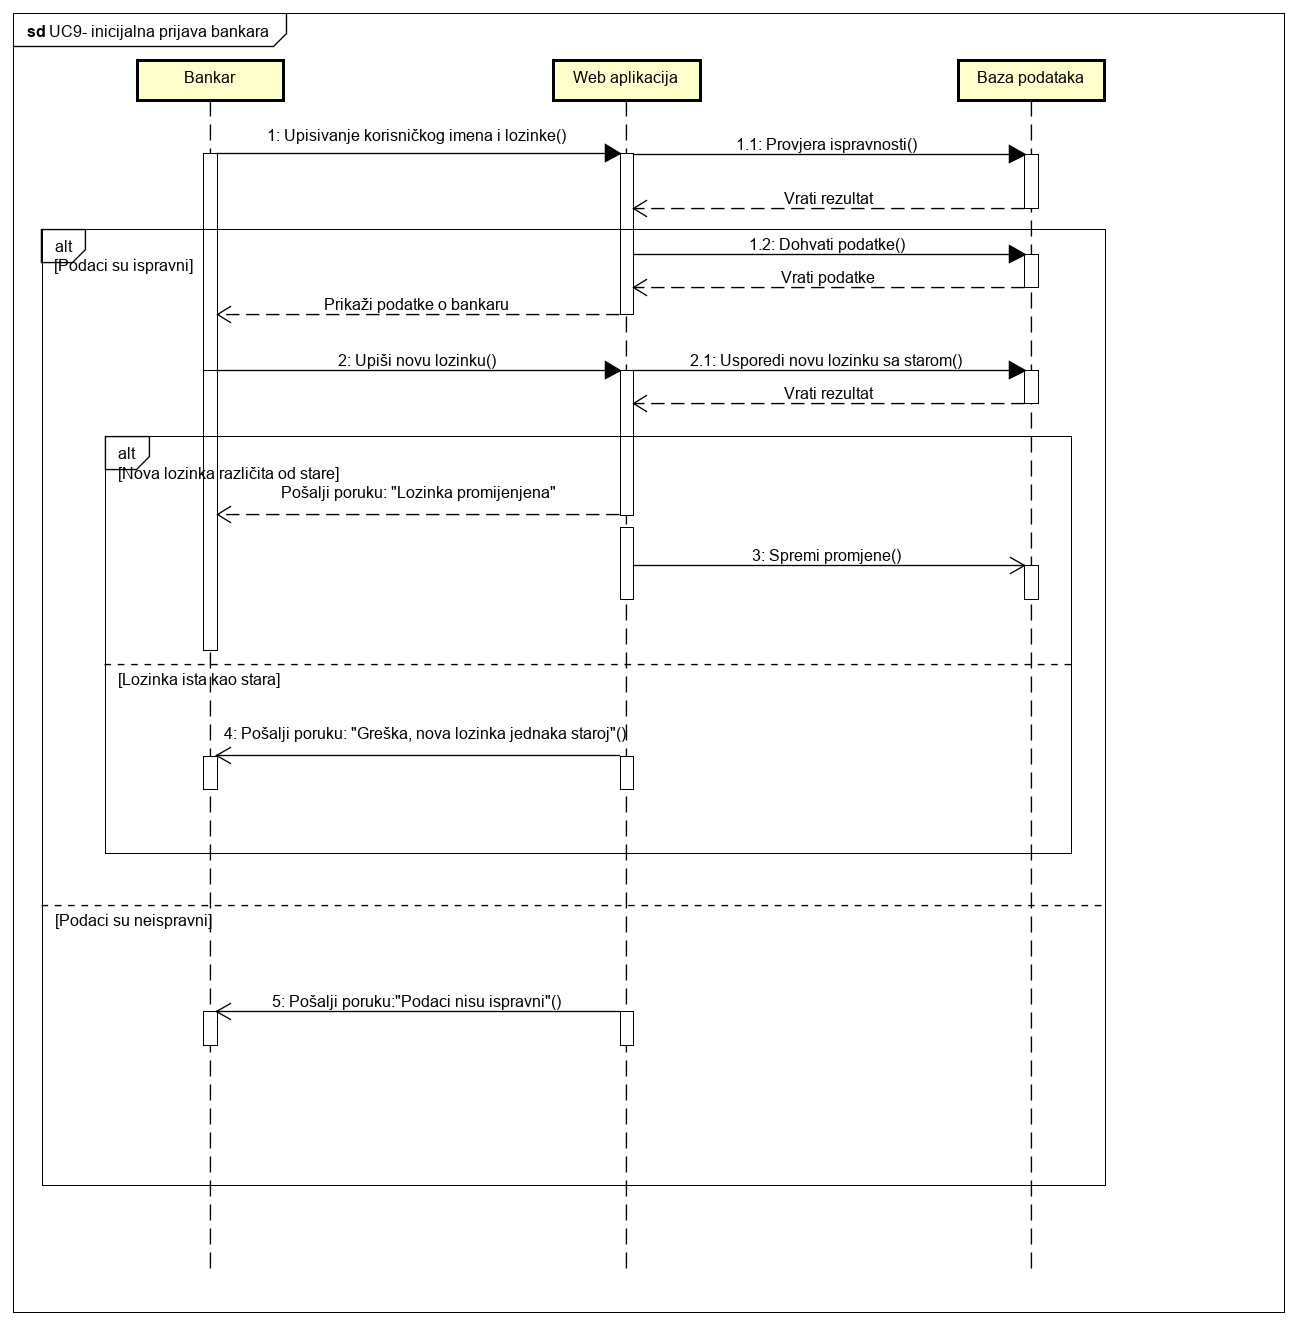
\includegraphics[scale=0.50]{slike/UC9.PNG}
					\centering
					\caption{Sekvencijski dijagram za UC9}
					\label{fig:uc9}
				\end{figure}
			\eject
			
			\noindent{\textbf{UC17 -  Ugovranje debitne kartice }}
			
			 Bankar upisuje klijentov OIB. Sustav provjerava ispravnost OIB-a u bazi podataka. Baza podataka vraća rezultate provjere. Ako je upisan OIB ispravan i postoji u bazi podataka, sustav dohvaća podatke o klijentu iz baze podataka i vraća ih bankaru na uvid. Bankar zatraži stvaranje kartice, sustav stvara karticu i promjene sprema u bazu podataka.Sustav šalje poruku bankaru da je kartica uspješno stvorena. Ukoliko je upisan OIB na početku bio neispravan i baza podataka je vratila negativne rezultate, sustav šalje poruku bankaru kako je upisan OIB neispravan.
			\eject
			
			\begin{figure}[H]
				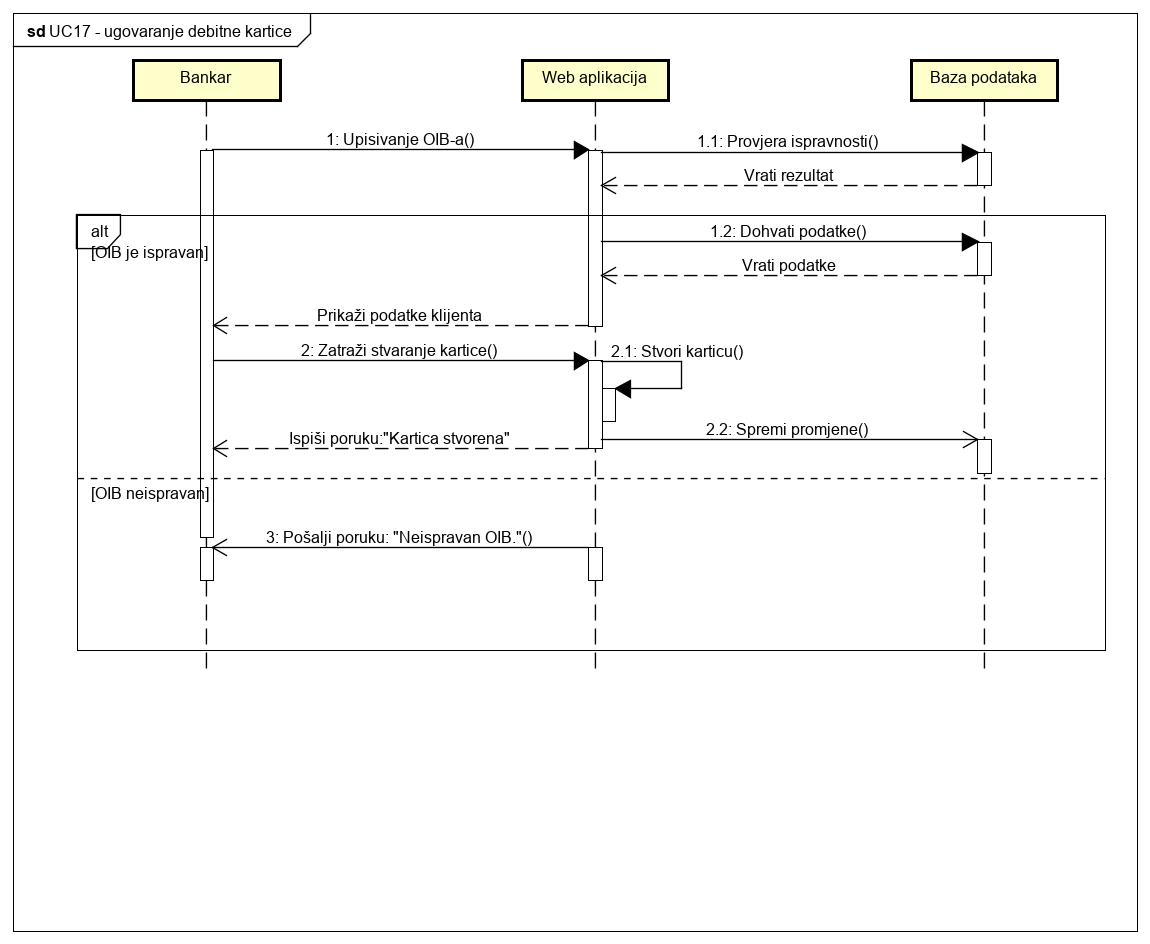
\includegraphics[scale=0.60]{slike/UC17.PNG}
				\centering
				\caption{Sekvencijski dijagram za UC17}
				\label{fig:uc17}
			\end{figure}
			\eject
			
			\noindent{\textbf{UC21 -  Ugovaranje kredita}}
			
			
			Bankar upisuje OIB u sustav. Web aplikacija provjerava ispravnost OIB-a s bazom podataka te baza podataka vraća rezultat. Ukoliko je OIB ispravan, sustav traži od baze podataka dohvaćanje klijentovih podataka. Baza podataka vraća podatke i sustav prikazuje bankaru podatke o klijentu. Bankar zatraži ugovaranje kredita, promjene se spremaju u bazu podataka i sustav šalje poruku da je zatraženo ugovaranje kredita. Ukoliko je OIB bio neispravan, bankar dobiva poruku od sustava da je OIB pogrešan.
			\eject
			
			\begin{figure}[H]
				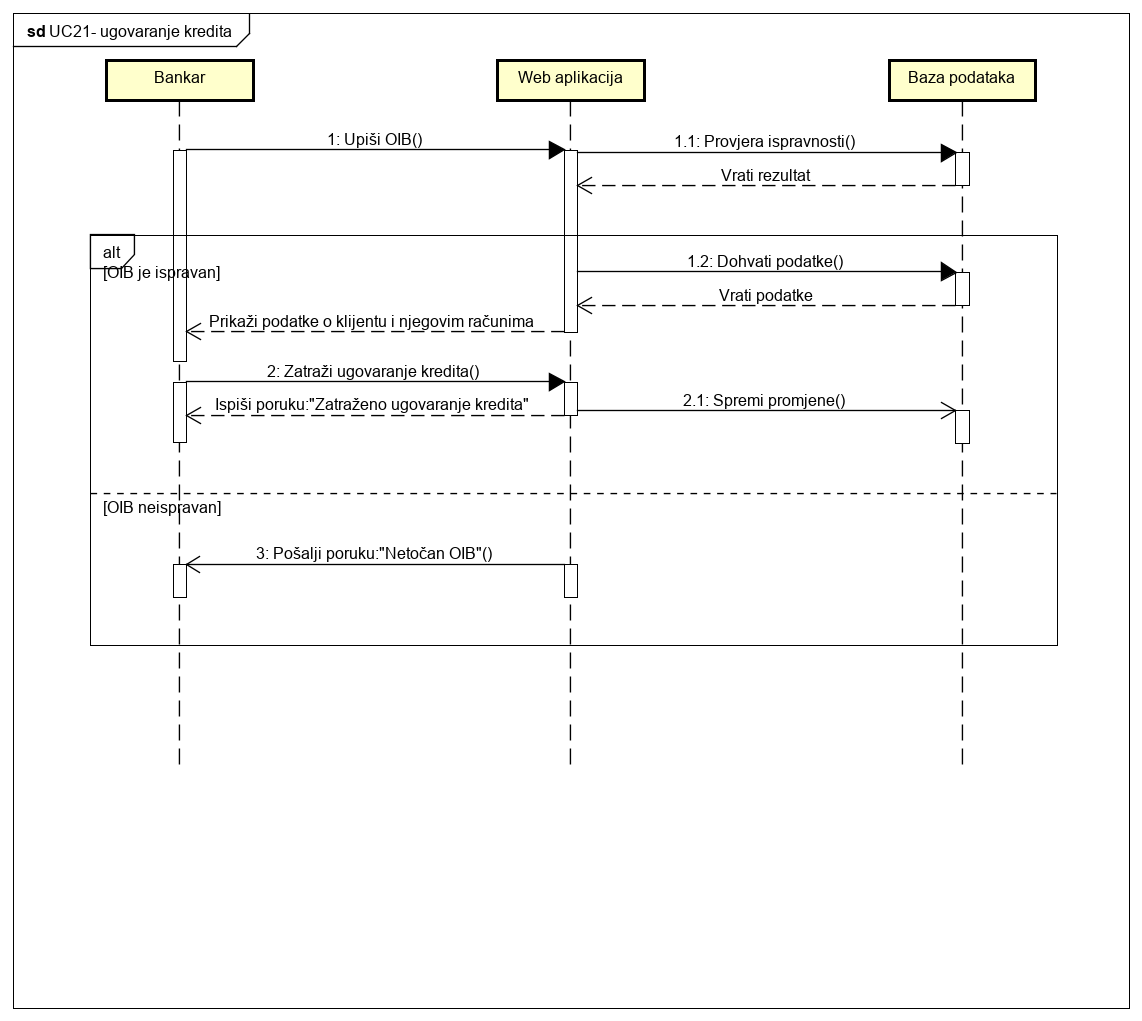
\includegraphics[scale=0.60]{slike/UC21.PNG}
				\centering
				\caption{Sekvencijski dijagram za UC21}
				\label{fig:uc21}
			\end{figure}
			\eject
			
			\noindent{\textbf{UC33 -  Registracija korisnika}}
			
			
			Kako bi se neregistrirani korisnik mogao registrirati, u sustav upisuje OIB i ključ koji je prethodno dobio od bankara. Sustav provjerava upisane podatke u bazi podataka te baza vraća rezulta. Ako su upisani podaci točni, sustav dohvaća podatke iz baze podataka i prikazuje iz klijentu. Klijent upisuje novo korisničko ime i lozinku te sustav opet provjerava zauzetost korisničkog imena u bazi podataka. Ukoliko je baza podataka vratila pozitivan rezultat, sustav sprema promjene u bazu podataka, a u slučaju negativnog rezultata baze podataka, sustav ispisuje poruku kojoj govori da je korisničko ime već zauzeto.
			\eject
			
			\begin{figure}[H]
				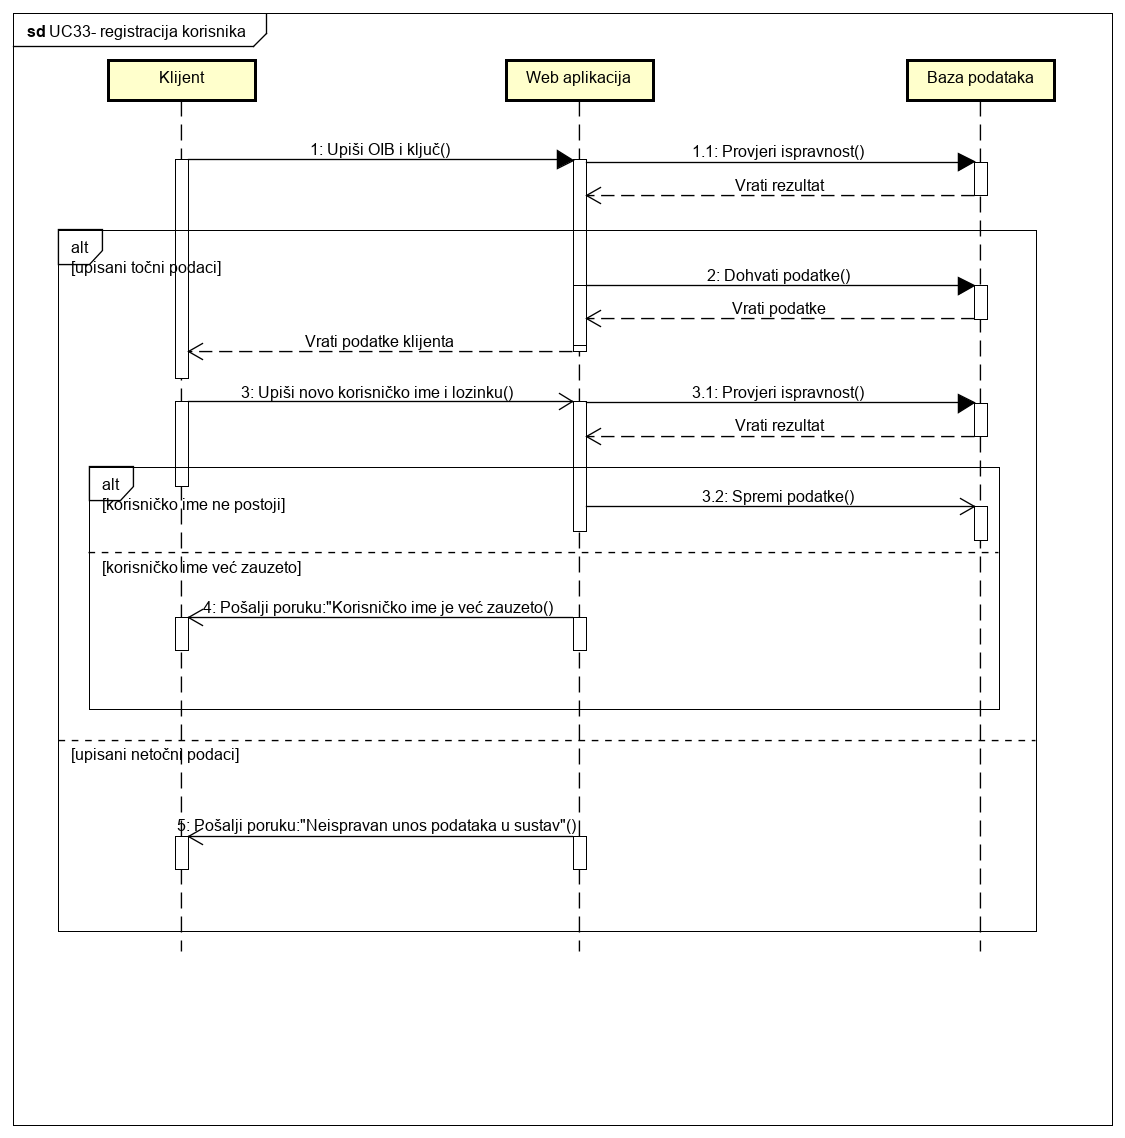
\includegraphics[scale=0.60]{slike/UC33.PNG}
				\centering
				\caption{Sekvencijski dijagram za UC33}
				\label{fig:uc33}
			\end{figure}
			\eject
			
	
		\section{Ostali zahtjevi}
			 
			 \begin{packed_item}
			 	\item Sustav mora podržavati rad više korisnika u stvarnom vremenu
			 	\item Aplikacija mora podržavati hrvatsku abecedu (dijakritičke znakove)
			 	\item Izvršavanje dijela programa u kojem se pristupa bazi podataka ne smije 
			 	trajati duže od nekoliko sekundi 
			 	\item Veza s bazom podataka mora biti kvalitetno zaštićena, brza i otporna na vanjske
			 	greške
			 	\item Nepravilno korištenje korisničkog sučelja ne smije narušiti funkcionalnost
			 	i rad sustava	
			 	\item Sustav treba biti jednostavan za upotrebu kako bi ga korisnici mogli koristiti
			 	bez opširnih uputa
			 	\item Nadogradnja sustava ne smije narušavati postojeće funkcionalnosti sustava
			 	\item Korisnički podaci jednog klijenta ne smiju biti vidljivi ostalim klijentima
			 	\item Klijent ne može mijenjati osobne podatke svog profila niti podatke o računima
			 	i karticama
			 	\item Svi računi moraju imati sliku profila
			 	\item Kao valuta se koristi HRK
			 	\item Svaki tekući račun treba imati dozvoljeno prekoračenje, a svaka kreditna kartica ugovoren limit.
			 	\item Jednom mjesečno korisnik treba dobiti izvod po svim transakcijskim
			 	računima i kreditnim karticama u PDF i XLS obliku
			 \end{packed_item}

	\chapter{Arhitektura i dizajn sustava}
		
		\textbf{\textit{dio 1. revizije}}\\

		\textit{ Potrebno je opisati stil arhitekture te identificirati: podsustave, preslikavanje na radnu platformu, spremišta podataka, mrežne protokole, globalni upravljački tok i sklopovsko-programske zahtjeve. Po točkama razraditi i popratiti odgovarajućim skicama:}
	\begin{itemize}
		\item 	\textit{izbor arhitekture temeljem principa oblikovanja pokazanih na predavanjima (objasniti zašto ste baš odabrali takvu arhitekturu)}
		\item 	\textit{organizaciju sustava s najviše razine apstrakcije (npr. klijent-poslužitelj, baza podataka, datotečni sustav, grafičko sučelje)}
		\item 	\textit{organizaciju aplikacije (npr. slojevi frontend i backend, MVC arhitektura) }		
	\end{itemize}

	
		

		

				
		\section{Baza podataka}
			
			
		Za potrebe našeg sustava koristit ćemo SQL relacijsku bazu podataka. Relacijska baza podataka najviše nam odgovara zbog olakšanog modeliranja događaja i entiteta iz stvarnog svijeta. Osnovna jedinka baze podataka je relacija, to jest tablica koja ima svoj naziv i potreban skup atributa. Zadaća baze podataka je brza i jednostavna pohrana, izmjena i dohvat podataka koje potom treba obraditi. Sve su relacije u bazi svedene na treću normalnu formu kako baza ne bi sadržavala redundantne podatke. Prilikom izrade baze podataka poslužili smo se PostgreSQL-om.
		Baza podataka ove aplikacije sastoji se od sljedećih entiteta:
		\begin{itemize}
			\item 	Profil
			\item 	KorisničkiRačun
			\item 	Uloga
			\item   TipUloge
			\item   Klijent
			\item   Djelatnik
			\item   Bankar
			\item   Administrator
			\item   SlužbenikZaOdobravanjeKredita
			\item   Banka
			\item   Kredit
			\item   Transakcija
			\item   Račun
			\item   VrstaRačuna
			\item   TekućiRačun
			\item   ŠtedniRačun
			\item   ŽiroRačun
			\item   Kartica
			\item   VrstaKartice
			\item   DebitnaKartica
			\item   KreditnaKartica
			\item   Kamata		
		\end{itemize}
		
			\subsection{Opis tablica}
			

				\textbf{Profil} Ovaj entitet sadrži sve važne informacije za pristup web aplikaciji. Sadrži atribute: ime, prezime, OIB, korisničko ime, adresa prebivališta, datum rođenja, e-mail adresa, slika profila i broj tipa uloge. Ovaj entitet u vezi je \textit{Zero-to-Many} s entitetom Korisnički račun preko korisničkog imena.  
				
				\begin{longtabu} to \textwidth {|X[6, l]|X[6, l]|X[20, l]|}
					
					\hline \multicolumn{3}{|c|}{\textbf{Profil }}	 \\[3pt] \hline
					\endfirsthead
					
					\hline \multicolumn{3}{|c|}{\textbf{Profil}}	 \\[3pt] \hline
					\endhead
					
					\hline 
					\endlastfoot
					
					\cellcolor{LightGreen}Ime & VARCHAR	&  	ime korisnika 	\\ \hline
					Prezime	& VARCHAR &  prezime korisnika 	\\ \hline 
					OIB & INT &  OIB korisnika \\ \hline 
					Korisničko ime & VARCHAR	&  	jedinstveni identifikator korisnika	\\ \hline 
					Adresa prebivališta & VARCHAR &   adresa korisnika      \\ \hline
					Datum rođenja & DATE & datum rođenja korisnika \\ \hline
					Email & VARCHAR & e-mail adresa korisnika \\ \hline
					Slika & LONGBLOB & slika korisnika \\ \hline
					Tip uloge & INT & broj tipa uloge \\ \hline
					 
					
					
				\end{longtabu}
			
			\textbf{Korisnički Račun}  Ovaj entitet sadrži sve važne informacije vezane za korisnički račun koji je dodijeljen svakom korisniku koji želi koristiti ovu web aplikaciju. Sadrži atribute: Korisničko ime, lozinku, OIB, ime i prezime korisnika te broj tipa uloge. Ovaj je entitet u vezi \textit{Many-to-Zero} s entitetom Profil preko korisničkog imena i u vezi \textit{One-to-One} s entitetom Uloga preko korisničkog imena.  
			
			\begin{longtabu} to \textwidth {|X[6, l]|X[6, l]|X[20, l]|}
				
				\hline \multicolumn{3}{|c|}{\textbf{Korisnički račun }}	 \\[3pt] \hline
				\endfirsthead
				
				\hline \multicolumn{3}{|c|}{\textbf{Korisnički račun}}	 \\[3pt] \hline
				\endhead
				
				\hline 
				\endlastfoot
				
				\cellcolor{LightGreen}Korisničko ime & VARCHAR	&  jedinstveni identifikator korisnika ( profil.korisničko ime) 	\\ \hline
				Lozinka	& VARCHAR &   hash lozinke	\\ \hline 
				OIB & INT & OIB korisnika (profil.oib)  \\ \hline
				Ime & VARCHAR &  ime korisnika (profil.ime)  \\ \hline 
				Prezime & VARCHAR	& prezime korisnika 		\\ \hline 
				\cellcolor{LightBlue} Tip uloge	& INT &  broj tipa uloge(profil.tip uloge) 	\\ \hline 
				
				
			\end{longtabu}
		
		\textbf{Uloga}  Ovaj entitet sadrži sve važne informacije vezane za ulogu koji je dodijeljen svakom korisniku koji želi koristiti ovu web aplikaciju. Sadrži atribute: Korisničko ime i broj tipa uloge. Ovaj je entitet u vezi \textit{One-to-One} s entitetom Korisnički račun preko korisničkog imena, u vezi \textit{One-to-One} s entitetom Tip Uloge preko broja tipa uloge.  
		
		\begin{longtabu} to \textwidth {|X[6, l]|X[6, l]|X[20, l]|}
			
			\hline \multicolumn{3}{|c|}{\textbf{Uloga}}	 \\[3pt] \hline
			\endfirsthead
			
			\hline \multicolumn{3}{|c|}{\textbf{Uloga}}	 \\[3pt] \hline
			\endhead
			
			\hline 
			\endlastfoot
			
			Korisničko ime & VARCHAR & Korisničko ime korisnika  \\ \hline
			\cellcolor{LightGreen}Tip uloge & INT	&  Broj tipa uloge	\\ \hline
			Naziv	& VARCHAR & Naziv uloge  	\\ \hline 
			
			 
			
			
		\end{longtabu}
	
		\textbf{Klijent} Ovaj entitet sadrži sve važne informacije vezane za klijenta. Sadrži atribute: ime, prezime, OIB, korisničko ime, lozinka, adresa prebivališta, datum rođenja, email, spol i slika. Ovaj entitet je u vezi \textit{One-to-Many} s entitetom Račun preko korisničkog imena, u vezi \textit{One-to-Many} s entitetom Kartica preko korisničkog imena korisnika. 
	
	\begin{longtabu} to \textwidth {|X[6, l]|X[6, l]|X[20, l]|}
		
		\hline \multicolumn{3}{|c|}{\textbf{Klijent}}	 \\[3pt] \hline
		\endfirsthead
		
		\hline \multicolumn{3}{|c|}{\textbf{Klijent}}	 \\[3pt] \hline
		\endhead
		
		\hline 
		\endlastfoot
		
			\cellcolor{LightGreen}Ime & VARCHAR	&  	ime klijenta 	\\ \hline
			Prezime	& VARCHAR &  prezime klijenta 	\\ \hline 
			OIB & INT &  OIB klijenta \\ \hline 
			Korisničko ime & VARCHAR	&  	jedinstveni identifikator korisnika	\\ \hline 
			Lozinka & VARCHAR & hash lozinke \\ \hline
			Adresa prebivališta & VARCHAR &   adresa klijenta      \\ \hline
			Datum rođenja & DATE & datum rođenja klijenta \\ \hline
			Email & VARCHAR & e-mail adresa korisnika \\ \hline
			Spol & VARCHAR(1) & spol klijenta \\ \hline
			Slika & LONGBLOB & slika korisnika \\ \hline
		
		
		
		
	\end{longtabu}

		\textbf{Djelatnik}  Ovaj entitet sadrži sve važne informacije koje su potrebne za djelatnika. Sadrži atribute: ime, prezime, OIB, korisničko ime, lozinku, adresu prebivališta, datum rođenja, e-mail, spol i broj tipa djelatnika te broj poslovnice banke. Ovaj entitet je u vezi \textit{Many-to-One} s entitetom Banka preko broja poslovnice banke u kojoj djelatnik radi. 
		
		\begin{longtabu} to \textwidth {|X[6, l]|X[6, l]|X[20, l]|}
			
			\hline \multicolumn{3}{|c|}{\textbf{Djelatnik}}	 \\[3pt] \hline
			\endfirsthead
			
			\hline \multicolumn{3}{|c|}{\textbf{Djelatnik}}	 \\[3pt] \hline
			\endhead
			
			\hline 
			\endlastfoot
			
			\cellcolor{LightGreen}Ime & VARCHAR	&  	ime djelatnika 	\\ \hline
			Prezime	& VARCHAR &  prezime djelatnika 	\\ \hline 
			OIB & INT &  OIB djelatnika \\ \hline 
			Korisničko ime & VARCHAR	&  	jedinstveni identifikator djelatnika	\\ \hline 
			Lozinka & VARCHAR & hash lozinke \\ \hline
			Adresa prebivališta & VARCHAR &   adresa klijenta      \\ \hline
			Datum rođenja & DATE & datum rođenja klijenta \\ \hline
			Email & VARCHAR & e-mail adresa korisnika \\ \hline
			Spol & VARCHAR(1) & spol klijenta \\ \hline
			Tip djelatnika & INT & Broj tipa uloge \\ \hline
			Broj banke & INT & Broj poslovnice banke\\ \hline
			
		
			
			
			
			
		\end{longtabu}
	
			\textbf{Bankar}    Ovaj entitet sadrži sve važne informacije za bankara. Sadrži sve atribute koje sadrži djelatnik te dodatno: broj tipa uloge i broj transakcije koje je proveo. Ovaj entitet u vezi je \textit{One-to-One} s entitetom djelatnik preko korisničkog imena bankara. Entitet bankar u vezi je i s entitetom Transakcija i Klijent vezom \textit{} preko broja transakcije. Isto tako, bankar je u vezi \textit{Many-to-Many} s entitetom Kredit preko broja kredita. Bankar je u vezi \textit{Many-to-One} s entitetom Administrator preko broja nadređenog bankaru.
			
			\begin{longtabu} to \textwidth {|X[6, l]|X[6, l]|X[20, l]|}
				
				\hline \multicolumn{3}{|c|}{\textbf{Bankar}}	 \\[3pt] \hline
				\endfirsthead
				
				\hline \multicolumn{3}{|c|}{\textbf{Bankar}}	 \\[3pt] \hline
				\endhead
				
				\hline 
				\endlastfoot
			
				Korisničko ime & VARCHAR	&  	jedinstveni identifikator bankara	\\ \hline 
				Broj tipa djelatnika & INT & broj tipa djelatnika \\ \hline
				Broj transakcije & INT & broj transakcije \\ \hline
				Broj kredita & LONG & Broj kredita koji ugovara\\ \hline
				Broj nadređenog & INT & broj tipa djelatnika nadređenog bankaru\\ \hline
				
				
				
				
				
			\end{longtabu}
		
		\textbf{Administrator}    Ovaj entitet sadrži sve važne informacije o administratoru. Administrator je zadužen za dodjeljivanje korisničkih računa i uloga bankara i službenika za odobravanje kredita. Sadrži atribute: korisničko ime, tip djelatnika i broj poslovnice banke. U vezi je \textit{Many-to-One} s entitetom Banka preko broja poslovnice banke u kojoj radi i u vezi \textit{One-to-Many} s entitetima Bankar i Službenik za odobravanje kredita preko broja tipa djelatnika.
		
		\begin{longtabu} to \textwidth {|X[6, l]|X[6, l]|X[20, l]|}
			
			\hline \multicolumn{3}{|c|}{\textbf{Administrator}}	 \\[3pt] \hline
			\endfirsthead
			
			\hline \multicolumn{3}{|c|}{\textbf{Administrator}}	 \\[3pt] \hline
			\endhead
			
			\hline 
			\endlastfoot
			
		 
			Korisničko ime & VARCHAR	&  	jedinstveni identifikator administratora	\\ \hline 
			Tip uloge & INT & broj tipa uloge \\ \hline
			Broj tipa djelatnika & INT & broj tipa djelatnika
			
			
			
			
		\end{longtabu}
	
		
				\textbf{Službenik za odobravanje kredita}   Ovaj entitet sadrži sve važne informacije koje su potrebne za ulogu službenika za odobravanje kredita. Sadrži atribute: korisničko ime, broj tipa uloge, broj poslovnice banke, broj nadređenog i broj kredita koji odobrava ili odbija. U vezi je \textit{Many-to-One} s entitetom Administrator preko broja tipa djelatnika nadređenog službeniku za odobravanje kredita. U vezi je \textit{Many-to-Many} s entitetom kredit preko broja kredita koji odobrava ili odbija. 
		
		\begin{longtabu} to \textwidth {|X[6, l]|X[6, l]|X[20, l]|}
			
			\hline \multicolumn{3}{|c|}{\textbf{Službenik za odobravanje kredita}}	 \\[3pt] \hline
			\endfirsthead
			
			\hline \multicolumn{3}{|c|}{\textbf{Službenik za odobravanje kredita}}	 \\[3pt] \hline
			\endhead
			
			\hline 
			\endlastfoot
			
			Korisničko ime & VARCHAR	&  	jedinstveni identifikator službenika	\\ \hline 
			Tip uloge & INT & broj tipa uloge\\ \hline
			Broj nadređenog & INT & broj tipa djelatnika nadređenog službeniku za odobravanje kredita\\ \hline
			Broj kredita & LONG & broj kredita\\ \hline
			
			
			
			
		\end{longtabu}
	
					\textbf{Banka}   Ovaj entitet sadrži sve važne informacije o poslovnici u kojoj rade djelatnici određene banke. Sadrži atribute: broj banke, naziv banke i adresa banke. U vezi je \textit{One-to-Many} s entitetom Djelatnik preko broja poslovnice banke i u vezi je \textit{Many-to-Many} s entitetom Kredit preko broja kredita koji daje određenom klijentu.  
			
			\begin{longtabu} to \textwidth {|X[6, l]|X[6, l]|X[20, l]|}
				
				\hline \multicolumn{3}{|c|}{\textbf{Banka}}	 \\[3pt] \hline
				\endfirsthead
				
				\hline \multicolumn{3}{|c|}{\textbf{Banka}}	 \\[3pt] \hline
				\endhead
				
				\hline 
				\endlastfoot
				
				Broj poslovnice & INT & broj poslovnice \\ \hline
				Adresa & VARCHAR & adresa banke \\ \hline
				Naziv & VARCHAR & naziv banke \\ \hline
				Broj kredita & LONG & broj kredita\\ \hline
				
				
				
				
			\end{longtabu}
		
			\textbf{Kredit}   Ovaj entitet sadrži sve važne informacije o kreditu koji klijent zatraži. Sadrži atribute: broj kredita, iznos, vrsta kredita, datum ugovaranja i vremenski period otplate kredita.U vezi je \textit{Many-to-One} s entitetom Bankar preko broja kredita i u vezi \textit{Many-to-One} s entitetom Klijent preko broja kredita. Isto tako, entitet Kredit u vezi je \textit{Many-to-One} s entitetom Službenik za odobravanje kredita preko broja kredita.
		
		\begin{longtabu} to \textwidth {|X[6, l]|X[6, l]|X[20, l]|}
			
			\hline \multicolumn{3}{|c|}{\textbf{Kredit}}	 \\[3pt] \hline
			\endfirsthead
			
			\hline \multicolumn{3}{|c|}{\textbf{Kredit}}	 \\[3pt] \hline
			\endhead
			
			\hline 
			\endlastfoot
			
			Broj kredita & LONG & broj kredita \\ \hline
			Iznos & DECIMAL (10, 2) & iznos kredita \\ \hline
			Vrsta & VARCHAR & vrsta kredita \\ \hline
			Datum ugovaranja & DATE & datum ugovaranja kredita \\ \hline
			Vremenski period otplate & INT & duljina otplate kredita \\ \hline
			
			
			
			
		\end{longtabu}
	
		
				\textbf{Transakcija}   Ovaj entitet sadrži sve važne informacije o transakcijama koje klijent želi provesti. Sadrži atribute: broj transakcije, broj računa terećenja, račun odobrenja, datum transakcije, iznos i ukupno stanje. Entitet Transakcija u vezi je \textit{Many-to-One} s entitetom Klijent preko broja transakcije i u vezi \textit{Many-to-One} s entitetom Bankar preko broja transakcije. Isto tako u vezi je \textit{Many-to-One} s entitetom Račun preko broja računa terećenja i broja računa odobrenja.
			
			\begin{longtabu} to \textwidth {|X[6, l]|X[6, l]|X[20, l]|}
				
				\hline \multicolumn{3}{|c|}{\textbf{Transakcija}}	 \\[3pt] \hline
				\endfirsthead
				
				\hline \multicolumn{3}{|c|}{\textbf{Transakcija}}	 \\[3pt] \hline
				\endhead
				
				\hline 
				\endlastfoot
				
				Broj transakcije & INT & broj transakcije \\ \hline
				Račun terećenja & INT & broj računa terećenja \\ \hline
				Račun odobrenja & INT & broj računa odobrenja \\ \hline
				Datum transakcije & DATE & datum transakcije \\ \hline
				Iznos & DECIMAL (10, 2) & iznos uplate \\ \hline
				Ukupno stanje & DECIMAL (10, 2) & ukupno stanje nakon transakcije \\ \hline
				
				
				
				
				
				
			\end{longtabu}
		
			\textbf{Račun}   Ovaj entitet sadrži sve važne informacije o računu koji ima klijent. Sadrži atribute: broj računa, OIB klijenta, datum otvaranja računa, stanje računa i vrsta računa. U vezi je  \textit{Many-to-One} s entitetom Klijent preko OIB-a klijenta. Entitet Račun također je u vezi \textit{Many-to-One} s entitetom Bankar preko korisničkog imena bankara i u vezi je \textit{One-to-Many} s entitetom Kartica preko broja kartice.
		
		\begin{longtabu} to \textwidth {|X[6, l]|X[6, l]|X[20, l]|}
			
			\hline \multicolumn{3}{|c|}{\textbf{Račun}}	 \\[3pt] \hline
			\endfirsthead
			
			\hline \multicolumn{3}{|c|}{\textbf{Račun}}	 \\[3pt] \hline
			\endhead
			
			\hline 
			\endlastfoot
			
			Broj računa & INT & broj računa \\ \hline
			OIB & INT & OIB klijenta \\ \hline
			Datum otvaranja & DATE & datum otvaranja računa \\ \hline
			Stanje & DECIMAL (10, 2) & trenutno stanje računa \\ \hline
			Korisničko ime bankara & VARCHAR & korisničko ime bankara koji je otvorio račun\\ \hline
			Broj kartice & LONG & broj kartice vezane uz račun\\ \hline
			
			
			
			
			
			
			
		\end{longtabu}
	
				\textbf{Vrsta računa}   Ovaj entitet sadrži sve važne informacije o vrsti računa koje neki klijent posjeduje. Sadrži atribute: broj vrste računa i naziv računa. U vezi je \textit{One-to-Many} s entitetima Tekući račun, Štedni račun i Žiro račun. 
			
			\begin{longtabu} to \textwidth {|X[6, l]|X[6, l]|X[20, l]|}
				
				\hline \multicolumn{3}{|c|}{\textbf{Vrsta računa}}	 \\[3pt] \hline
				\endfirsthead
				
				\hline \multicolumn{3}{|c|}{\textbf{Vrsta računa}}	 \\[3pt] \hline
				\endhead
				
				\hline 
				\endlastfoot
				
				Vrsta računa & INT & Broj vrste računa \\ \hline
				Naziv računa & VARCHAR & Naziv vrste računa \\ \hline
				
				
				
				
				
				
				
			\end{longtabu}
		
		
			\textbf{Tekući račun}   Ovaj entitet sadrži sve važne informacije koje nam trebaju za izgradnju tekućeg računa. Sadrži atribute: broj računa, broj vrste računa i prekoračenje. U vezi je \textit{One-to-One} s entitetom Račun preko broja računa i u vezi \textit{One-to-One} s entitetom Vrsta računa preko broja vrste računa. 
		
		\begin{longtabu} to \textwidth {|X[6, l]|X[6, l]|X[20, l]|}
			
			\hline \multicolumn{3}{|c|}{\textbf{Tekući račun}}	 \\[3pt] \hline
			\endfirsthead
			
			\hline \multicolumn{3}{|c|}{\textbf{Tekući račun}}	 \\[3pt] \hline
			\endhead
			
			\hline 
			\endlastfoot
			
			Broj računa & LONG & broj tekućeg računa \\ \hline
			Broj vrste računa & INT & broj vrste računa\\ \hline
			Prekoračenje & DECIMAL(10,2) & iznos prekoračenja računa \\ \hline
		
			
			
			
			
			
			
		\end{longtabu}
	
		
			
		\textbf{Štedni račun}  
		
		\begin{longtabu} to \textwidth {|X[6, l]|X[6, l]|X[20, l]|}
			
			\hline \multicolumn{3}{|c|}{\textbf{Štedni račun}}	 \\[3pt] \hline
			\endfirsthead
			
			\hline \multicolumn{3}{|c|}{\textbf{Štedni račun}}	 \\[3pt] \hline
			\endhead
			
			\hline 
			\endlastfoot
			
			Broj računa & INT & broj štednog računa \\ \hline
			OIB & INT & OIB klijenta \\ \hline
			Datum otvaranja & DATE & datum otvaranja računa \\ \hline
			Stanje & DECIMAL (10, 2) & trenutno stanje računa \\ \hline
			Kamatna stopa & DECIMAL(2, 2) & iznos kamatne stope \\ \hline
			Datum zatvaranja & DATE & datum zatvaranja računa \\ \hline
			
			
			
			
			
			
			
		\end{longtabu}
		
		
			
	
		

			
			
			\subsection{Dijagram baze podataka}
				\textit{ U ovom potpoglavlju potrebno je umetnuti dijagram baze podataka. Primarni i strani ključevi moraju biti označeni, a tablice povezane. Bazu podataka je potrebno normalizirati. Podsjetite se kolegija "Baze podataka".}
			
			\eject
			
			
		\section{Dijagram razreda}
		
			\textit{Potrebno je priložiti dijagram razreda s pripadajućim opisom. Zbog preglednosti je moguće dijagram razlomiti na više njih, ali moraju biti grupirani prema sličnim razinama apstrakcije i srodnim funkcionalnostima.}\\
			
			\textbf{\textit{dio 1. revizije}}\\
			
			\textit{Prilikom prve predaje projekta, potrebno je priložiti potpuno razrađen dijagram razreda vezan uz \textbf{generičku funkcionalnost} sustava. Ostale funkcionalnosti trebaju biti idejno razrađene u dijagramu sa sljedećim komponentama: nazivi razreda, nazivi metoda i vrste pristupa metodama (npr. javni, zaštićeni), nazivi atributa razreda, veze i odnosi između razreda.}\\
			
			\textbf{\textit{dio 2. revizije}}\\			
			
			\textit{Prilikom druge predaje projekta dijagram razreda i opisi moraju odgovarati stvarnom stanju implementacije}
			
			
			
			\eject
		
		\section{Dijagram stanja}
			
			
			\textbf{\textit{dio 2. revizije}}\\
			
			\textit{Potrebno je priložiti dijagram stanja i opisati ga. Dovoljan je jedan dijagram stanja koji prikazuje \textbf{značajan dio funkcionalnosti} sustava. Na primjer, stanja korisničkog sučelja i tijek korištenja neke ključne funkcionalnosti jesu značajan dio sustava, a registracija i prijava nisu. }
			
			
			\eject 
		
		\section{Dijagram aktivnosti}
			
			\textbf{\textit{dio 2. revizije}}\\
			
			 \textit{Potrebno je priložiti dijagram aktivnosti s pripadajućim opisom. Dijagram aktivnosti treba prikazivati značajan dio sustava.}
			
			\eject
		\section{Dijagram komponenti}
		
			\textbf{\textit{dio 2. revizije}}\\
		
			 \textit{Potrebno je priložiti dijagram komponenti s pripadajućim opisom. Dijagram komponenti treba prikazivati strukturu cijele aplikacije.}
	\chapter{Implementacija i korisničko sučelje}
		
		
		\section{Korištene tehnologije i alati}
		
			\textbf{\textit{dio 2. revizije}}
			
			 \textit{Detaljno navesti sve tehnologije i alate koji su primijenjeni pri izradi dokumentacije i aplikacije. Ukratko ih opisati, te navesti njihovo značenje i mjesto primjene. Za svaki navedeni alat i tehnologiju je potrebno \textbf{navesti internet poveznicu} gdje se mogu preuzeti ili više saznati o njima}.
			
			
			\eject 
		
	
		\section{Ispitivanje programskog rješenja}
			
			\textbf{\textit{dio 2. revizije}}\\
			
			 \textit{U ovom poglavlju je potrebno opisati provedbu ispitivanja implementiranih funkcionalnosti na razini komponenti i na razini cijelog sustava s prikazom odabranih ispitnih slučajeva. Studenti trebaju ispitati temeljnu funkcionalnost i rubne uvjete..}
	
			
			\subsection{Ispitivanje komponenti}
			\textit{Potrebno je provesti ispitivanje jedinica (engl. unit testing) nad razredima koji implementiraju temeljne funkcionalnosti. Razraditi \textbf{minimalno 6 ispitnih slučajeva} u kojima će se ispitati redovni slučajevi, rubni uvjeti te izazivanje pogreške (engl. exception throwing). Poželjno je stvoriti i ispitni slučaj koji koristi funkcionalnosti koje nisu implementirane. Potrebno je priložiti izvorni kôd svih ispitnih slučajeva te prikaz rezultata izvođenja ispita u razvojnom okruženju (prolaz/pad ispita). }
			
			
			
			\subsection{Ispitivanje sustava}
			
			 \textit{Potrebno je provesti i opisati ispitivanje sustava koristeći radni okvir Selenium\footnote{\url{https://www.seleniumhq.org/}}. Razraditi \textbf{minimalno 4 ispitna slučaja} u kojima će se ispitati redovni slučajevi, rubni uvjeti te poziv funkcionalnosti koja nije implementirana/izaziva pogrešku kako bi se vidjelo na koji način sustav reagira kada nešto nije u potpunosti ostvareno. Ispitni slučaj se treba sastojati od ulaza (npr. korisničko ime i lozinka), očekivanog izlaza ili rezultata, koraka ispitivanja i dobivenog izlaza ili rezultata.\\ }
			 
			 \textit{Izradu ispitnih slučajeva pomoću radnog okvira Selenium moguće je provesti pomoću jednog od sljedeća dva alata:}
			 \begin{itemize}
			 	\item \textit{dodatak za preglednik \textbf{Selenium IDE} - snimanje korisnikovih akcija radi automatskog ponavljanja ispita	}
			 	\item \textit{\textbf{Selenium WebDriver} - podrška za pisanje ispita u jezicima Java, C\#, PHP koristeći posebno programsko sučelje.}
			 \end{itemize}
		 	\textit{Detalji o korištenju alata Selenium bit će prikazani na posebnom predavanju tijekom semestra.}
			
			\eject 
		
		
		\section{Dijagram razmještaja}
			
			\textbf{\textit{dio 2. revizije}}
			
			 \textit{Potrebno je umetnuti \textbf{specifikacijski} dijagram razmještaja i opisati ga. Moguće je umjesto specifikacijskog dijagrama razmještaja umetnuti dijagram razmještaja instanci, pod uvjetom da taj dijagram bolje opisuje neki važniji dio sustava.}
			
			\eject 
		
		\section{Upute za puštanje u pogon}
		
			\textbf{\textit{dio 2. revizije}}\\
		
			 \textit{U ovom poglavlju potrebno je dati upute za puštanje u pogon (engl. deployment) ostvarene aplikacije. Na primjer, za web aplikacije, opisati postupak kojim se od izvornog kôda dolazi do potpuno postavljene baze podataka i poslužitelja koji odgovara na upite korisnika. Za mobilnu aplikaciju, postupak kojim se aplikacija izgradi, te postavi na neku od trgovina. Za stolnu (engl. desktop) aplikaciju, postupak kojim se aplikacija instalira na računalo. Ukoliko mobilne i stolne aplikacije komuniciraju s poslužiteljem i/ili bazom podataka, opisati i postupak njihovog postavljanja. Pri izradi uputa preporučuje se \textbf{naglasiti korake instalacije uporabom natuknica} te koristiti što je više moguće \textbf{slike ekrana} (engl. screenshots) kako bi upute bile jasne i jednostavne za slijediti.}
			
			
			 \textit{Dovršenu aplikaciju potrebno je pokrenuti na javno dostupnom poslužitelju. Studentima se preporuča korištenje neke od sljedećih besplatnih usluga: \href{https://aws.amazon.com/}{Amazon AWS}, \href{https://azure.microsoft.com/en-us/}{Microsoft Azure} ili \href{https://www.heroku.com/}{Heroku}. Mobilne aplikacije trebaju biti objavljene na F-Droid, Google Play ili Amazon App trgovini.}
			
			
			\eject 
	\chapter{Zaključak i budući rad}

		 Zadatak našeg tima bio je razvoj web i mobilne aplikacije za online bankarstvo. Realizacija projekta podijeljena je u dvije faze.
		 
		 U prvoj fazi projekta okupljen je tim za razvoj aplikacije. Na prvom sastanku definirana je ideja projekta te izvršena podjela uloga članovima tima. 
		 U prvoj fazi definiran je i napravljen temelj cijelog sustava. Značajan dio dokumentacije napisan u ovoj fazi projekta uvelike je olakšao daljnji rad pri realizaciji aplikacije. Pisanjem funkcionalnih i nefunkcionalnih zahtjeva, crtanjem uml dijagrama, izradom modela baze podataka pomoglo se članovima tima zaduženim za implementaciju aplikacije.
		 
		 U drugoj fazi projekta naglasak se stavlja na implementaciju aplikacije. Članovi tima zaduženi za backend i frontend intenzivno rade na realizaciji aplikacije kako bi uspjeli implementirati sve dogovorene funkcionalnosti aplikacije. Ostatak tima bio je zadužen za crtanje preostalih uml dijagrama, testiranje i dovršavanje dokumentacije. Zahvaljujući dobro definiranim temeljima projekta u prvoj fazi dokumentacije, ubrzali smo fazu implementacije te spriječili moguće pogreške. Članovi tima stekli su znanja o raznim tehnologijama i alatima za koje su pokazali interes i s kojima će se možda susresti u budućnosti.
		 
		 Nakon gotove aplikacije i dalje postoji prostor za usavršavanje. U budućnosti bilo bi potrebno doraditi mobilnu aplikaciju kako bi sadržavala sve funkcionalnosti kao i web aplikacija.
		 
		 Zadovoljni smo postignutim rezultatom te stječenim znanjima kroz ovaj projekt. Osim susretanja sa novim tehnologijama i sudjelovanju u procesu implementacije aplikacije, stekli smo osjećaj rada u timu te važnosti dobre organizacije i pravilne raspodjele poslova.
		
		\eject 
	\chapter*{Popis literature}
		\addcontentsline{toc}{chapter}{Popis literature}
	 	
 		\textbf{\textit{Kontinuirano osvježavanje}}
	
		\textit{Popisati sve reference i literaturu koja je pomogla pri ostvarivanju projekta..}
		
		
		\begin{enumerate}
			
			
			\item  Oblikovanje programske potpore, FER ZEMRIS, \url{http://www.fer.hr/predmet/opp}
			
			\item  I. Sommerville, "Software engineering", 8th ed, Addison Wesley, 2007.
			
			\item  T.C.Lethbridge, R.Langaniere, "Object-Oriented Software Engineering", 2nd ed. McGraw-Hill, 2005.
			
			\item  I. Marsic, Software engineering book``, Department of Electrical and Computer Engineering, Rutgers University, \url{http://www.ece.rutgers.edu/~marsic/books/SE}
			
			\item  The Unified Modeling Language, \url{https://www.uml-diagrams.org/}
			
			\item  Astah Community, \url{http://astah.net/editions/uml-new}
		\end{enumerate}
		
		 
	
	
	\begingroup
	\renewcommand*\listfigurename{Indeks slika i dijagrama}
	%\renewcommand*\listtablename{Indeks tablica}
	%\let\clearpage\relax
	\listoffigures
	%\vspace{10mm}
	%\listoftables
	\endgroup
	\addcontentsline{toc}{chapter}{Indeks slika i dijagrama}


	
	\eject 
		
	\chapter*{Dodatak: Prikaz aktivnosti grupe}
		\addcontentsline{toc}{chapter}{Dodatak: Prikaz aktivnosti grupe}
		
		\section*{Dnevnik sastajanja}
		
		\begin{packed_enum}
			\item  sastanak
			
			\item[] \begin{packed_item}
				\item Datum: u ovom formatu: 4. listopada 2019.
				\item Prisustvovali: M. Bačić, M. Anušić, D. Milošević, M. Milički, K. Gudelj, M. Vučemilo, L. Bastalić
				\item Teme sastanka:
				\begin{packed_item}
					\item  Upoznavanje
					\item  Razrada prijedloga projektnog zadatka
					\item  Podjela uloga u projektu
				\end{packed_item}
			\end{packed_item}
			
			\item  sastanak
			\item[] \begin{packed_item}
				\item Datum: u ovom formatu: 9. listopada 2019.
				\item Prisustvovali: M. Bačić, M. Anušić, D. Milošević, M. Milički, K. Gudelj, M. Vučemilo, L. Bastalić
				\item Teme sastanka:
				\begin{packed_item}
					\item  Inicijalni sastanak s asistentom
					\item  Razgovor oko prijedloga zadatka
				\end{packed_item}
			\end{packed_item}
		
			\item  sastanak
			\item[] \begin{packed_item}
				\item Datum: u ovom formatu: 15. listopada 2019.
				\item Prisustvovali: M. Bačić, M. Anušić, D. Milošević, M. Milički, K. Gudelj, M. Vučemilo, L. Bastalić
				\item Teme sastanka:
				\begin{packed_item}
					\item  Budući da je prijedlog zadatka odobren, konkretne upute dobivene od asistenta
				\end{packed_item}
			\end{packed_item}
		
			\item  sastanak
			\item[] \begin{packed_item}
				\item Datum: u ovom formatu: 22. listopada 2019.
				\item Prisustvovali: M. Bačić, M. Anušić, D. Milošević, K. Gudelj, L. Bastalić
				\item Teme sastanka:
				\begin{packed_item}
					\item  Povratna informacija od asistenta za trenutni napredak
				\end{packed_item}
			\end{packed_item}
		
			\item  sastanak
			\item[] \begin{packed_item}
				\item Datum: u ovom formatu: 24. listopada 2019.
				\item Prisustvovali:  M. Bačić, M. Anušić, D. Milošević, M. Milički, K. Gudelj, M. Vučemilo, L. Bastalić
				\item Teme sastanka:
				\begin{packed_item}
					\item  Povratna informacija od asistenta za trenutni napredak
				\end{packed_item}
			\end{packed_item}
			
			%
			
		\end{packed_enum}
		
		\eject
		\section*{Tablica aktivnosti}
		
			\begin{longtabu} to \textwidth {|X[7, l]|X[1, c]|X[1, c]|X[1, c]|X[1, c]|X[1, c]|X[1, c]|X[1, c]|}
								
				\cline{2-8} \multicolumn{1}{c|}{\textbf{}} &     \multicolumn{1}{c|}{\rotatebox{90}{\textbf{Matija Bačić }}} & \multicolumn{1}{c|}{\rotatebox{90}{\textbf{Klara Gudelj }}} &	\multicolumn{1}{c|}{\rotatebox{90}{\textbf{Lorena Bastalić }}} &	\multicolumn{1}{c|}{\rotatebox{90}{\textbf{Magda Milički }}} &
				\multicolumn{1}{c|}{\rotatebox{90}{\textbf{Marija Vučemilo }}} &
				\multicolumn{1}{c|}{\rotatebox{90}{\textbf{Marko Anušić }}} &	\multicolumn{1}{c|}{\rotatebox{90}{\textbf{Dominik Milošević }}} \\ \hline 
				\endfirsthead
				
			
				\cline{2-8} \multicolumn{1}{c|}{\textbf{}} &     \multicolumn{1}{c|}{\rotatebox{90}{\textbf{Matija Bačić }}} & \multicolumn{1}{c|}{\rotatebox{90}{\textbf{Klara Gudelj }}} &	\multicolumn{1}{c|}{\rotatebox{90}{\textbf{Lorena Bastalić }}} &	\multicolumn{1}{c|}{\rotatebox{90}{\textbf{Magda Milički }}} &
				\multicolumn{1}{c|}{\rotatebox{90}{\textbf{Marija Vučemilo }}} &
				\multicolumn{1}{c|}{\rotatebox{90}{\textbf{Marko Anušić }}} &	\multicolumn{1}{c|}{\rotatebox{90}{\textbf{Dominik Milošević }}} \\ \hline  
				\endhead
				
				
				\endfoot
							
				 
				\endlastfoot
				
				Upravljanje projektom 		& 3 & 1.5 & 1.5 & 1.5 & 1.5 & 1.5 & 1.5 \\ \hline
				Opis projektnog zadatka 	& 2 &  &  &  &  &  & \\ \hline
				
				Funkcionalni zahtjevi       & 0.5 &  &  &  &  &  & 2.5 \\ \hline
				Opis pojedinih obrazaca 	& 2 & 6 & 6 &  &  &  &  \\ \hline
				Dijagram obrazaca 			& 3 &  &  &  &  & 2 &  \\ \hline
				Sekvencijski dijagrami 		&  &  &  & 4.5 &  &  &  \\ \hline
				Opis ostalih zahtjeva 		&  &  &  &  & 3 &  &  \\ \hline

				Arhitektura i dizajn sustava	 &  &  &  &  &  &  &  \\ \hline
				Baza podataka				&  &  &  &  &  &  &   \\ \hline
				Dijagram razreda 			&  &  &  &  &  &  &   \\ \hline
				Dijagram stanja				&  &  &  &  &  &  &  \\ \hline
				Dijagram aktivnosti 		&  &  &  &  &  &  &  \\ \hline
				Dijagram komponenti			&  &  &  &  &  &  &  \\ \hline
				Korištene tehnologije i alati 		&  &  &  &  &  &  &  \\ \hline
				Ispitivanje programskog rješenja 	&  &  &  &  &  &  &  \\ \hline
				Dijagram razmještaja			&  &  &  &  &  &  &  \\ \hline
				Upute za puštanje u pogon 		&  &  &  &  &  &  &  \\ \hline 
				Dnevnik sastajanja 			&  &  &  &  &  &  &  \\ \hline
				Zaključak i budući rad 		&  &  &  &  &  &  &  \\  \hline
				Popis literature 			&  &  &  &  &  &  &  \\  \hline
				&  &  &  &  &  &  &  \\ \hline \hline
				\textit{Dodatne stavke kako ste podijelili izradu aplikacije} 			&  &  &  &  &  &  &  \\ \hline
				\textit{npr. izrada početne stranice} 				&  &  &  &  &  &  &  \\ \hline 
				\textit{izrada baze podataka} 		 			&  &  &  &  &  &  & \\ \hline 
				\textit{spajanje s bazom podataka} 							&  &  &  &  &  &  &  \\ \hline
				\textit{back end} 							&  &  &  &  &  &  &  \\  \hline
				 							&  &  &  &  &  &  &\\  \hline
				
				
			\end{longtabu}
					
					
		\eject
		\section*{Dijagrami pregleda promjena}
		
		\textbf{\textit{dio 2. revizije}}\\
		
		\textit{Prenijeti dijagram pregleda promjena nad datotekama projekta. Potrebno je na kraju projekta generirane grafove s gitlaba prenijeti u ovo poglavlje dokumentacije. Dijagrami za vlastiti projekt se mogu preuzeti s gitlab.com stranice, u izborniku Repository, pritiskom na stavku Contributors.}
		
	


\end{document}